\chapter{Relational Database, Data Mining, and Statistical
Theory}\label{chap:review}

The aims of this chapter are to provide the requisite
background to be able to read the thesis as a self-contained body of
work as well as enabling the reader to appreciate this research within
the wider fields of both relational database theory and data mining.

In Section~\ref{sec:db_for_dm} we present the relationship of this
work to both database and data mining theory. 
In Section~\ref{sec:relmod} we introduce the relational database theoretic
concepts relevant to this thesis and in Section~\ref{sec:datmin}
introduce the area of data mining, concentrating firstly on dependency data
mining so that the reader can fully appreciate the context of
Chapter~\ref{chap:numdep} and then temporal data mining for the
background of Chapters~\ref{chap:templog}
and~\ref{chap:tempresult}. In later chapters we will refer to 
the definitions presented in~\ref{sec:relmod} and~\ref{sec:datmin}
as and when they are initially used.

\section{Database Theory for Data Mining}\label{sec:db_for_dm}
\index{Data Mining!and Database Theory}
There has been significant work in the data mining community on the
mining of {\em data dependencies}, both in standard \cite{psm93,km95} and
temporal environs \cite{bwj96}. Much of this concentrates solely
on the discovery process, in effect working totally within a machine
learning (ML) context, i.e. \cite{she91}; scant regard is paid to the
database theory upon which the dependencies are based. Though we
do not question the quality of this work because of this omission we
believe that NDs which fit into the
relational model, both for design and, as we show in this thesis, data
mining, are a valuable tool. Until recently, much data mining research
was disjoint from database 
theory, based within statistics or machine learning though there is
now a body of work on unifying these areas \cite{cha98}; this thesis
requires an appreciation of both.
We introduce the background material on
database theory in Section~\ref{sec:relmod} to clarify
later work on Armstrong relations and the chase procedure, a
theorem proving tool for FDs in a relation, as well as our use of indefinite
information for the consistency problem. Theoretical work on FD
behaviour has directly led to the 
creation of numerous data mining methodologies which we introduce
in~\ref{subsec:fdmining}.  Section~\ref{sec:relmod} concludes with a
presentation of 
temporal databases and dependencies.

Section~\ref{sec:datmin} introduces aspects of dependency data mining,
including a discussion of the relationship to NDs. We provide a
discussion of measures based 
on aspects of FD theory in~\ref{subsec:fdmining}. We then introduce
temporal databases and dependencies before moving on to temporal data
mining and rule discovery from time series, closely
related to work in Chapters~\ref{chap:templog} and~\ref{chap:tempresult}.
This section concludes with a brief overview of sampling in data
mining followed by an informal introduction to resampling, useful for
later work presented on indefinite and temporal relations.

\section{Relational Database Theory}\label{sec:relmod}
\index{Relational Database|see{Relational Data Model}}

We now present the relational database theory required within this
thesis. The reader is referred to
\cite{databasefound,atze93,Maier83,Ullm88} for a complete coverage of
the area.

\subsection{The Relational Model}
\index{Relational Data Model}

In 1970, E. F. Codd introduced the relational model \cite{cod70}, with
relations as the data structure,  so
that database users need not concern themselves with the physical
storage of data.  This allowed independence between programs and their
machine representations by providing a sound basis for describing the
structure of data and operations for data manipulation without the
need for consideration of the internal machine
representation. Subsequently other data models have been developed,
including the Entity-Relationship model, for high level conceptual
database modelling, and object-oriented data models
\cite{kim90,databasefound}. The latter were primarily developed to
combat the growing requirements for complex data manipulation; we do
not make further reference to these data models and remain within the
confines of the relational model in this thesis. Its universality and
ease of data 
manipulation does not require further justification. We now formalise the
relational model.

\index{Universe}
\begin{definition}[Universe]
\begin{rm}
A universe $\cal U$ is a finite, fixed set of symbols that represent the 
column names which can appear within a relation.  They are referred to
as attributes. 
\end{rm} 
\end{definition}

\index{Attribute Domain}
\begin{definition}[Attribute Domain]
\begin{rm}
The domain of an attribute A $\in \cal U$, denoted by DOM(A), is the
countable set
of possible values which can be members of A.  This is the set
of values which can appear in a column of A.
\end{rm}
\end{definition}
\index{Relation Schema}
\index{Relation}
\begin{definition}[Relation Schema and Relation]
\begin{rm}
A relation schema R is a subset of the universe $\cal U$.  The elements
of a relation schema are denoted by $\{$ A$_1$, $\ldots$, A$_n$ $\}$.
A {\em tuple} over R is an element of DOM(A$_1$) $\times \ldots \times$
DOM(A$_n$), where $\times$ refers to the cartesian product.  An instance
of a relation over R is a finite set of tuples defined over R.
\end{rm}
\end{definition}

A relation consists of a finite set of tuples where each tuple
represents an entity.  A relation is therefore simply an entity set. 
Each tuple can be considered a row if we assume
the table representation of a relational database.
\index{Database Schema}
\begin{definition}[Database Schema and Database]
\begin{rm}
A Database Schema over $R$ is a finite set of relation schema $\{$ R$_1$,
$\ldots$, R$_n$ $\}$.  A database over $R$ is a finite set $d$ = $\{ r_1,
\ldots, r_n \}$ such that each $r_i \in d$ is a relation over R$_i \in
R$.
\end{rm}
\end{definition}

The relational algebra is presented by Codd \cite{cod70} in the context of
deriving desired result relations from other relations.  The operations include
{\em selection}, {\em projection}, defined below, {\em join}, {\em
union}, {\em difference}, and
{\em renaming};  all are defined in
\cite{databasefound,atze93,Date95,Maier83,Ullm88}.
\index{Projection}
\begin{definition}[Projection]
\begin{rm}
The projection of an R-tuple $t$ onto a set of attributes Y $\subseteq$
R, denoted by $t[$Y$]$ (also called the Y-value of $t$), is the
restriction of $t$ to the attributes in Y.  The projection of a
relation $r$ onto Y, denoted as $\pi_{\rm Y}$($r$),
is defined by $\pi_{\rm Y}$($r$) = \{ t[Y] $\mid$ t $\in$ $r$ \}.
\end{rm}
\end{definition}

We now move on to the representation of constraints in the relational
model required to ensure the maintenance of integrity within a
database. Data mining now often uses such constraints and constraint
approximations to discover previously unknown and non-trivial
information \cite{kdd96}.


\subsection{Functional Dependencies}
\index{Integrity Constraints}
			\index{Data Dependencies}
			\index{Functional Dependency}
			\index{Determination}
			\index{Key}
			\index{Functional Independency}
			\index{Axiomatisation}
		 	\index{Soundness}
			\index{Completeness}
Integrity constraints, or data dependencies, allow a database to have
associated with it an intended meaning or semantics for the tuples
within the database.  The most common
constraint is the FD introduced in
\cite{cod72}, its prevailing application in practice is as
a key dependency.  FDs were given a {\em sound} and
{\em complete} axiomatisation in \cite{Arms74}.  We note that {\em
soundness} implies that each dependency, which is derived using a
finite number of applications of an axiomatisation from a given set,
holds. {\em Completeness} implies that valid each dependency which holds can be
derived using the axiomatisation. FDs
are restricted first order logic (FOL) sentences shown in
\cite{sdpf81} to be equivalent to Horn clause statements, relating
determinations to logical implication \cite{fag77,logicfound,mak87}. 
There has been extensive work on the theory of FDs,
of which some seminal contributions are
\cite{Arms74,fag77,bb79,sdpf81}. Although work on FD theory has somewhat
exhausted itself there has recently been extensive work in data mining for
approximating FDs \cite{Mann92,sf93,bb95,hkp98}.

\begin{definition}[Data Dependency]
\begin{rm}
A data dependency is a restricted integrity constraint incorporating a
(specified) property that is to be satisfied by all instances of the database
schema.
\end{rm}
\end{definition}

Dependencies within the relational model allow for the incorporation of a more
complex semantics via meta-data representations. We now formalise the
FD, its axiom system, and the closure of FD attribute sets. 

\index{Functional Dependency}
\begin{definition}[Functional Dependency (FD)]
\begin{rm}
A {\em functional dependency} over R (or simply an FD)
is a statement of the form X $\to$ Y, where X, Y $\subseteq$ R.
\end{rm}
\end{definition}
\medskip
 
 F {\em is known as a set of FDs over} R and X $\to$ Y 
{\em is  a single FD over} R. We denote logical implication by $\models$.
A key dependency is an FD of the form X $\to$ R for some X $\subseteq$
R. 
\index{Functional Dependency!Satisfaction}
\begin{definition}[Satisfaction of an FD]\label{def:sat}
\begin{rm}
Given $r$,  a definite relation over R,
an FD X $\to$ Y is {\em satisfied} in $r$,
denoted by $r \models$ X $\to$ Y, whenever
$\forall t_1, t_2 \in$ $r$, if $t_1$[X] = $t_2$[X] then $t_1$[Y] = $t_2$[Y].
A set of FDs F is {\em satisfied} in $r$,
denoted by $r \models$ F, whenever
$\forall$ X $\to$ Y $\in$ F, $r \models$ X $\to$ Y.
\end{rm}
\end{definition}
\medskip
\index{Armstrong's axioms!for FDs}
FDs obey a set of axioms, shown to be sound and complete in
\cite{Arms74}, which are:
\begin{definition}[Armstrong's Axioms for functional dependencies]
\begin{rm}
Given a relation schema R and X,Y,Z $\subseteq$ R:
{\line
\begin{description}
\item[Reflexivity] If Y $\subseteq$ X, then X $\to$ Y
\item[Augmentation] If X $\to$ Y then XZ $\to$ YZ
\item[Transitivity] If X $\to$ Y and Y $\to$ Z, then X $\to$ Z
\end{description}
}
\end{rm}
\end{definition}


\index{Closure!of an attribute set}

\begin{definition}[Closure of an attribute set]
\begin{rm}
Given a set F of FDs over a set of attributes X the closure of X
under F, denoted X$^+$, is the set $\{$ A $\in$ R $\mid$ F $\models$ X $\to$ A $\}$
\end{rm}
\end{definition}

X$_{\rm F}^+$ refers to the closure of X with respect to F, that is
the set of all attributes A $\in$ R such that X $\to$ A holds in F.
We define F$^\star$ to be the closure of F such that trivial
FDs of the form X $\to$ Y, where Y $\subseteq$ X, are excluded.

\begin{definition}[Non-trivial closure]
\begin{rm}
F$^\star$ = $\{$ X $\to$ Y $\mid$ XY $\subseteq$ R and Y $\subseteq$
X$_{\rm F}^+$ $-$  X $\}$
\end{rm}
\end{definition}

\begin{definition}[Closure of a set of attribute sets]
\begin{rm}
Given an FD set F we denote the closure of all possible
attribute sets under F by CL(F). This is defined as
CL(F) = $\{$ X $\mid$ X $\subseteq$ R and X$_{\rm F}^+$ = X $\}$
\end{rm}
\end{definition}

Note that the schema R is always included in the closure of attribute
sets for any FD set. The next lemma shows that F$^\star$ and 
CL(F) are equivalent in characterising a set of FDs F. The
non-trivial closure is relevant in data mining measures,
discussed in Section~\ref{subsec:fdmining}.

\begin{lemma}
\begin{rm}
Given two sets of FDs, F and G, we then prove 
G$^\star$ $\subseteq$ F$^\star \equiv$ CL(G) $\supseteq$ CL(F)
\end{rm}
\end{lemma}

{\em Proof. (if) }
Assume, to the contrary, that CL(G) $\not\supseteq$ CL(F).
Therefore $\exists$ X $\in$ CL(F) such that X $\not\in$ CL(G), implying
that X is not closed in G. 
Then X$_{\rm G}^+$ = XY, for some attribute set Y.
 This implies that X $\to$ Y is in G but
not in F, yet G$^\star \subseteq$ F$^\star$, leading to a
contradiction.

\smallskip
{\em (only-if)}
Assume, to the contrary, that G$^\star \not\subseteq$ F$^\star$. 
Then $\exists$ X $\to$ Y $\in$ G$^\star$ such that X $\to$ Y $\not\in$
F$^\star$. 
Then Y $\subseteq$ X$_{\rm G}^+$ but Y $\not\subseteq$ X$_{\rm F}^+$, 
and so X$^+_{\rm G} \not=$ X$^+_{\rm F}$.
Given that CL(G) $\supseteq$ CL(F) it must be the case that 
any closed set in F
must be closed in G, and so we have a contradiction. $\Box$

\medskip
\index{Closure!of a set of FDs}
\begin{definition}[Closure of a set of FDs]
\begin{rm}
Given an FD set F we denote the closure of F by F$^+$. 
This is defined as
\begin{displaymath}
\mbox{F}^+ = \{\mbox{X} \to \mbox{Y} \mid \mbox{XY} \subseteq \mbox{R}
\mbox{ and } \mbox{F} \models \mbox{X}
\to \mbox{Y}  \}
\end{displaymath}
\end{rm}
\end{definition}


An algorithm to compute the closure of a set of FDs is in 
\cite{databasefound,atze93} which runs in time linear to the size of
the set FDs. The
concept of a maximal set is now introduced; its data mining
applications will be briefly discussed in
Section~\ref{subsec:fdmining} and Chapter~\ref{chap:numdep}.
\index{Maximal Set}
\begin{definition}[Maximal Set]
\begin{rm}
Given X, a subset of schema R, and A $\in$ X then
a set Y $\subseteq$ X is a {\em maximal} set for A, if F
$\not\models$ Y $\to$ A and for any
Z $\subseteq$ X such that Y $\subset$ Z we have F $\models$ Z $\to$ A
\end{rm}
\end{definition}

\begin{definition}[The set of all maximal sets]
\begin{rm}
$max$(F,X,A) = $\{$ Y $\subseteq$ X $\mid$ Y is a maximal set such that
F $\not\models$ Y $\to$ A $\}$.  If F is understood from the context then it
is written simply $max$(X,A); $max$(X) denotes the union of $max$(X,A)
where A $\in$ X.
\end{rm}
\end{definition}


A maximal set is an attribute set X which for some attribute A is
a largest possible set {\em not} determining A. We also define
generator sets. The generator function omits those sets from the
closure of an attribute set which can be formed by the intersection of
other sets in the closure to obtain a more concise
representation. Theorem 13.1 of \cite{Mann92} shows that $max$(X) = GEN(X).
\index{Generator Function!and Maximal Sets}
\begin{definition}[The generator function]
\begin{rm}
The generator function produces a set for X such that
GEN(X) = $\{$ Y $\in$ CL(X) $\mid$ Y $\subset \bigcap \{$ W $\in$
CL(X) $\mid$ Y $\subset$ W $\}\}$
\end{rm}
\end{definition}

We now define the cover of a set of dependencies, useful for
discovering equivalent FD sets.

\index{Cover!of a dependency set}

\begin{definition}[Cover of a set of Dependencies]
\begin{rm}
Given sets F and G of FDs, F is a {\em cover} of G
if F$^+$ = G$^+$. A {\em cover} G is minimal for F if there does not
exist a cover H of F such that $\mid$ H $\mid$ $<$ $\mid$ G $\mid$. A
minimal cover is necessarily nonredundant,  
that is, $\forall d \in$ G we have  G $\backslash \{ d \} \not\models
d$, though nonredundancy does not imply minimality. 
\end{rm}
\end{definition}

\begin{example}
\begin{rm}
From \cite{mr92}, the set F = $\{$ A $\to$ BC, B $\to$ AD, CD $\to$ E,
E $\to$ CD $\}$ and the set  G = $\{$ A $\to$ BE, B $\to$ A, CD $\to$
E, E $\to$ CD $\}$ are equivalent. This is proven by showing that G
$\models$ F and F $\models$ G.  The non-trivial 
cases are showing that F $\models$ A $\to$ E and G $\models$ $\{$ A
$\to$ C, B $\to$ D $\}$. To illustrate, A $\to$ C may be shown to hold
from G as we know A $\to$ E holds, by transitivity A $\to$ CD
holds, and therefore A $\to$ C is known to be satisfied by G. 
\end{rm}
\end{example}

To test if two covers, F and G, are equivalent we can check that
every X $\to$ Y $\in$ F is satisfied in G and vice versa.  Using the
algorithm presented in \cite{mr92} this can be done in time $O( \mid$ F
$\mid \|$ G $\| + \mid$ G $\mid \|$ F $\|)$, where $\|$ X $\|$ denotes
the number of attributes in X including repetitions. Alternatively, we
can check for 
equivalence of the maximal sets. We now introduce some notation to aid
the reading of the next section.
\index{Agreement set}
\begin{definition}[Agreement set of two tuples]
\begin{rm}
Given a relation $r$ over R, where $t_1$,$t_2$ are
two tuples in $r$ the agreement set is defined as
$ag(t_1, t_2)$ $=$ $\{$ B $\in$ R $\mid$ $t_1[$B$]$ $=$
$t_2[$B$]$$\}$. \newline 
The disagreement set is defined dually, disag($t_1$,$t_2$) = R
$\backslash ag(t_1, t_2) $.
\end{rm}
\end{definition}

Given an attribute A in disag(a,b) let X be the disagreement set of all
attributes for tuples a and b apart from A, i.e. X = disag(a,b) $\backslash \{$A$\}$.  
Then any set in the left-hand side of A must contain at least one
attribute of X. Why is this so?  Let us assume that it does not hold and
that for a member of the left-hand side of A an attribute of X is not
contained.  This implies, however, that there exist two tuples which disagree
on A when they have the same left-hand side.  Obviously this violates F and so is
not the case. X is therefore said to be a necessary set for A, used in
dependency mining \cite{Mann92}.

\begin{definition}[Agreement set of a relation]
\begin{rm}
Given a relation $r$ over attribute set R, the agreement set is defined as
$agr(r) = \{ ag(t_1,t_2) \mid$ $t_1,t_2 \in r \}$.
\end{rm}
\end{definition}


We now define Armstrong Relations (AR) and
follow this with a discussion of database design and its relationship
to data mining.

\subsection{Armstrong Relations}\index{Armstrong Relations}


\cite{Arms74} introduced the concept of an {\em Armstrong relation}:  

\begin{definition}[Armstrong Relation]
\begin{rm}
An Armstrong relation for F is a relation $r$ which satisfies F$^+$
and is such
that for every FD $\sigma \not\in {\rm F}^+$ for which  F$^+ \not\models
\sigma$, then $r$ violates $\sigma$.
\end{rm}
\end{definition}

In theory, Armstrong relations \cite{fag82,bdfs84,dt95,gl90,lev95,mr86}
serve as ``ideal'' example relations, since they satisfy exactly the set of
all logical consequences of the set of FDs specified, say F.
Thus an Armstrong relation provides an example for all FDs
that are logically implied by F and a counterexample for all 
those FDs that are not logically implied by F.
One of the problems with Armstrong relations is that, in general,
their cardinality is exponential in the size of F and the set of attributes, R,
over which F is defined \cite{bdfs84}. An Armstrong relation for a
set of FDs, if
deterministically generated \cite{Mann92}, always provides
the same resulting relation. It would be highly desirable if varying Armstrong relations
of different domain and tuple sizes may be generated as a side effect of 
the forming of example relations.

\medskip

\cite{fag82} presents a survey of Armstrong Databases  including
descriptions of the techniques for generating Armstrong Relations from
a set of FDs.  
These are: (1) Use {\em disjoint union } to create an isomorphic copy of each
relation and then form the union of all of the tuples in all of the
relations. For each FD $\sigma$ which is not a logical consequence of
the relations create a relation $r_\sigma$ which obeys F but not
$\sigma$. Then form the union for all {\em standard} FDs, where the
left hand side is non-empty, to give an
AR.  (2) Create {\em agreement
sets}. The agreement set is formed such that
GEN(F) $\subseteq agr(r) \subseteq$ CL(F). \cite{bdfs84} construct
an Armstrong relation by firstly computing the closure of the FD set
F, CL(F), and then constructing a relation such that $agr(r)$ =
CL(F). (3) {\em Direct
products }(used by \cite{gm85a} to prove no Horn clause
representation exists for NDs). A relation is created for each $\sigma$ outside
of CL(F) which violates $\sigma$ and satisfies CL(F). The direct
product of these is then formed. (4) Use the {\em chase procedure},
presented in Section~\ref{subsec:rev_chase}. Given
an Armstrong relation which obeys an FD set
F and violates all FDs outside of CL(F) form a model where all
FDs are violated using the chase which can cause new tuples and/or
constants to be added to the database. We shall see in
Chapter~\ref{chap:numdep} how an evolutionary technique using mutation
and guided by ND
satisfaction may often generate Armstrong relations \cite{cl96,cl98c}.

\medskip

\cite{fv83} shows that an Armstrong database may be generated for a
set of inclusion  
dependencies and standard FDs.  An inclusion dependency
states that if some combination of values occurs in one part of a
database it  must also occur in another part.  
\medskip

Lemma 3.1 \cite{bdfs84} shows that if $\Sigma$ is a set of FDs and $\sigma$ a
single FD such that $\Sigma \not\models \sigma$ then there exists a two tuple
relation that obeys $\Sigma$ but not $\sigma$.  A by-product of this result is
that it is always possible to add a tuple to a relation $r$ satisfying
$\Sigma$ which
violates $\sigma$.  A deficiency of deterministic processes for AR
generation are that
only one specific Armstrong relation is ever returned for a given FD
set. \cite{bdfs84} present an analysis on the upper and lower bounds of the
size of an Armstrong Relation based on the number of distinct entries 
in the relation, referred to as the generator sets which \cite{mr86} 
later refine. 
\cite{mr86} show that the size of a minimal Armstrong relation for a
normalised  scheme R depends strongly on the number of keys for R.
The possible exponential size of a minimal Armstrong relation depends
only on the number of dependencies, and not on the number of attributes. 

An Armstrong relation should be as small as possible, as should the
set of values used, though the smaller the relation the more difficult
it becomes for the designer to locate all of the anomalies as opposed
to an Armstrong relation which lists all examples of dependency
violations in a pairwise format.\\ 

\subsection{Relational Database Design}\label{subsec:reldbdes}
\index{Relational Database Design}
\index{Database Design|see {Relational Database Design}}
\index{Referential Integrity}
\index{Normalisation}
			\index{Redundancy}
			\index{Normal Form}
			
We now mention relational
database design related to work presented in
Chapter~\ref{chap:numdep}. Informally, database design attempts to
remove redundancy and facilitate querying by the use of normalisation.
A relation can be 
constructed to adhere to a series of increasingly restrictive normal forms introduced so as to prevent redundancy and (update) anomalies within the
database, discussed in
\cite{cod72,databasefound,atze93,Date95,Maier83,Ullm88}.  

\medskip

Keys provide the only method for tuple identification  in the standard
relational model, and they are
therefore central to the retrieval of information and good database design. There are many key
related properties whose determination is computationally intractable
\cite{lo78}. We now present the superkey class, used within Boyce-Codd
Normal Form.

\index{SuperKey}
\index{BCNF|see{Boyce Codd Normal Form}}
\index{Boyce Codd Normal Form}
\begin{definition}[SuperKey]
\begin{rm}
Given a relation scheme R and a set  $\Sigma$ of FDs which apply to it, a  set of attributes X is a superkey for R if the FD X $\to$ R $\in \Sigma^+$.
\end{rm}
\end{definition}

\begin{definition}[Boyce Codd Normal Form]\label{def:bcnf}
\begin{rm}
Given a relation scheme R and a set of FDs $\Sigma$ which apply to it, R is in Boyce Codd Normal Form (BCNF) if for every non-trivial FD X $\to$ A $\in \Sigma^+$, X is a superkey.
\end{rm}
\end{definition}


We assume that all relations discussed in this thesis
satisfy first normal form (1NF), where each relation is flat, and
present a database or relation satisfying BCNF as the ideal normal form,
where each non-trivial FD has a superkey as its left hand side. BCNF
attempts to 
overcome the deficiencies in 3NF by dropping the constraint that {\em
non-prime} attributes, those not in any key, which are allowed on the
right hand side of FDs may violate the normal
form . \cite{bb79}
present an analysis method to achieve a BCNF relation by splitting
relations successively which violate BCNF, though this procedure is
not guaranteed to be constraint preserving.  A non-mathematical
treatment of normal 
forms is given in \cite{ken83} which are then extended for temporal 
relations in \cite{jss92}. 
\medskip
\index{Example Relation}

\cite{sm81} introduced the
idea of example relations generated from a set of FDs and MVDs  for 
database design purposes. 
They present a design technique which attempts to provide the
database designer an iterative method of obtaining the FD set which
most {\em characterises} a relation.  More recently  \cite{mr86,mr92},
approached various database 
design problems with the goal of formalising methods and tools to
produce schemas with specific properties. They 
introduce the technique of using example relations within the design
process, notably as ``an application of ARs'', by presenting an
algorithm to deterministically generate ARs for the benefit of the
database designer.  \cite{bdfs84} note how an
Armstrong relation, perhaps generated automatically from a set of FDs, is of
much use in the design process from an application point of view.
Automated database design has 
been seen as a goal for dependency theory \cite{bv84}.

\medskip

In \cite{cl98c}, summarised in Chapter~\ref{chap:numdep}, we present
 a probabilistic extension of this work, 
 allowing the database designer to view many different example
 relations, though not necessarily ARs, for any given FD set specified
 over R. The size of the relation is governed by the database designer.
 \cite{mr86} state,  ``A good example
 relation should not leave the designer any illusions about what can
 be stored in the database.'' Our algorithm for generating example
 relations achieves this. It is based on the following loop
which we envisage during the database design process:
\begin{enumerate}
\item The database designer specifies a set of FDs, F, 
 the maximum number of tuples in the example relation, $m$, and
the maximum domain size, $d$, for a relation. (The designer
has the options of specifying $m$ and $d$ so that relations
of different structure can be viewed.)
\item A random example relation satisfying F, 
having at most $m$ tuples, and a domain ranging
from 2 to $d$ values is generated. The quality,
in terms of its proximity to that of an Armstrong relation, for the 
FD set is measured and returned to the designer.
\item The database designer either accepts F or modifies the parameters
F, $m$ and $d$, 
and then returns to step (2).
\end{enumerate}

Two aspects of this work are discussed subsequently; the
evolutionary hill climbing algorithm which uses NDs in a hill climbing
fashion to obtain a relation satisfying an FD set is presented in
Chapter~\ref{chap:numdep} and the {\em
quality} function used to obtain a proximity to an Armstrong relation
for the output, which may be viewed as the data mining component of
this work, is introduced in~\ref{subsec:rev_fd_sim}.

\subsection{The Chase Procedure}\label{subsec:rev_chase}
\index{Chase Procedure!for FDs}

If we have an attribute set R, an FD set F over R and a relation
$r$ which does not satisfy F, $r \not\models$ F, we can use the
chase procedure to modify $r$ so that it satisfies F. This technique
is known as the chase, introduced in \cite{mms79} and generalised 
to tuple and equality generating dependencies in \cite{bv84}. We
assume in algorithm~\ref{alg:chase}, without
loss of generality,  that our
domains are {\em linearly ordered}.

{\renewcommand{\baselinestretch}{1}
\begin{figure}[ht]
\begin{center}
\fbox{\begin{minipage}{14cm}
\begin{algorithm}[{\rm CHASE}($r$, {\rm F})]\label{alg:chase}
\begin{rm}
\begin{tabbing}
t1\=t2\=t3\=t4\=t5\=t6\= \kill \\
\na.  \> \> {\bf begin} \\
\sa.  \> \> \> Result := $r$; \\
\sa.  \> \> \> Tmp := $\emptyset$; \\
\sa.  \> \> \> {\bf while} Tmp $\not=$ Result {\bf do} \\
\sa.  \> \> \> \> Tmp := Result; \\
\sa.  \> \> \> \> {\bf if} $\exists X \to Y \in$ F and $\exists t_1,
t_2 \in$ Result \\
\> \> \> \>  \> such that $t_1$[X] = $t_2$[X] but $t_1$[Y] $\not=$
$t_2$[Y] {\bf then} \\
\sa.  \> \> \> \> \> \> $\forall A \in$ Y$-$X, $t_1$[A], $t_2$[A] := max($t_1$[A], $t_2$[A]); \\
\sa.  \> \> \> \> {\bf end if} \\
\sa.  \> \> \> {\bf end while} \\
\sa. \> \> \> {\bf return} Result;  \\
\sa. \> \> {\bf end.}
\end{tabbing}
\end{rm}
\end{algorithm}
\end{minipage}}
\end{center}
\caption{\label{rev:fd_chase} The Chase procedure for FDs}
\end{figure}
}

Given that NDs and FDs are expressible in First-Order Logic (FOL) any
FOL proof procedure may be applied. The chase is however suitably
specialised for FDs avoiding costly theorem proving
procedures. Additionally, the 
chase procedure is a decision procedure in that it always halts.
We can discover the closure of a set of attributes
X by creating a two-tuple relation which agrees on X and disagrees
on all other attributes. After the chase procedure halts (proven to
occur in \cite{mms79}) the agreement set in the relation $r$ consists
of exactly the closure of X.  We illustrate this with a small
example for the FD set F = $\{$ T $\to$ H, H $\to$ C $\}$ and the
relation $r_{1}$ in Table~\ref{tab:befcha}. We wish to
obtain the closure of T, shown in Table~\ref{tab:aftcha} after
application of the chase where T$^+$ = THC.


{\line
\begin{table}[ht]
\begin{minipage}[b]{6cm}
\begin{center}
\begin{tabular}{|c|c|c|} \hline
 T & H & C \\ \hline
 2 & 1 & 1 \\
 2 & 2 & 4 \\  \hline
\end{tabular}
\end{center}
\caption{\label{tab:befcha}$r_{1}$ before the chase}
\end{minipage}
\hfill
\begin{minipage}[b]{6cm}
\begin{center}
\begin{tabular}{|c|c|c|} \hline
 T & H & C \\ \hline
 2 & 2 & 4 \\  \hline
\end{tabular}
\end{center}
\caption{\label{tab:aftcha}$r_{1}$ after the chase, T$^+$ = THC}
\end{minipage}
\end{table}
}

In Chapter~\ref{chap:numdep} we generalise the concept of
the equality generating chase to cover NDs and in Chapter~\ref{chap:consistency} we extend it
to accept relations which contain indefinite information. Examples of
the chase in use are given in \cite{databasefound,Mann92}. In
\cite{ler86} it is noted that the chase turns a database consisting of
extensional and intensional data into one containing extensional data only.


\subsection{Numerical Dependency Theory}\label{subsec:rev_ndtheory}
\index{Numerical Dependency}
\index{Cardinality Constraint}
\index{Branching Dependency}
\index{Scalability!of NDs}
\index{Boolean Dependency}

\cite{gm85a,gm85b} introduced the concept of NDs as
extensions of FDs for providing the database designer
with additional flexibility.  They have a clear intuitive semantics
which can easily be accommodated for many database representation
issues, including cardinality constraints.


\begin{definition}[Numerical Dependency (ND)]
\begin{rm}
A {\em numerical dependency} over R (or simply an ND)
is a statement of the form X $\to^k$ Y, where X, Y $\subseteq$ R and $k \ge 1$.
\end{rm}
\end{definition}
\smallskip
\index{branching factor|see{Numerical Dependency}}
\index{Numerical Dependency!branching factor}
We let N be {\em a set of NDs over} R and X $\to^k$ Y 
{\em is a single ND over} R, with $k \ge 1$.
Intuitively, an ND X $\to^k$ Y is satisfied in a definite relation $r$ over R,
if each X-value in $r$ is associated with at most $k$ Y-values in $r$;
when $k = 1$ then the ND X $\to^1$ Y reduces to the FD X $\to$ Y. For
an ND X $\to^k$ Y we refer to $k$ as the branching factor. The 
satisfaction of X $\to^k$ Y with $k > 1$ is equivalent to the
satisfaction of a Functional Independency \cite{gl90}.
NDs are generalisations of FDs which
allow an attribute set to uniquely determine up to $k$ different attribute
set values, noting that $k = 1$ in the case of FDs. For any given FD
set F and a relation $r$ the set of all possible approximations forms a
{\em complete lattice} \cite{dp90}; this is the basis for a metric we define
in Chapter~\ref{chap:numdep} and use for how well an ND set
approximates F in Chapter~\ref{chap:consistency}. 

\index{Numerical Dependency!Satisfaction}

\begin{definition}[Satisfaction of an ND]\label{def:sat-nd}
\begin{rm}
Given a definite relation $r$ over R,
an ND X $\to^k$ Y is {\em satisfied} in $r$,
denoted by $r \models$ X $\to^k$ Y, whenever
$\forall t_1, t_2, \ldots, t_k, t_{k+1} \in$ r, if 
$t_1$[X] = $t_2$[X] = $\ldots$ = $t_k$[X] = $t_{k+1}$[X] then 
$\exists i,j$ such that $1 \le i < j \le k+1$
and $t_i$[Y] = $t_j$[Y].
A set of NDs N is {\em satisfied} in $r$,
denoted by $r \models$ N, whenever
$\forall$ X $\to^k$ Y $\in$ N, $r \models$ X $\to^k$ Y.
\end{rm}
\end{definition}

We now present an
example of the application of NDs in Table~\ref{tbl:1.0}  in a
teaching relation $PLAN$(Lecturer, Course).  The intended semantics for
this relation is that a lecturer can teach up to, but not more than, 2
different courses, written as Lecturer $\to^2$ Course.
 
{\line
\begin{table}[ht]
\begin{center}
\begin{tabular}{||l|l||} \hline
{\bf Lecturer} & {\bf Course} \\ \hline
 Mark &  C320 \\
 Robin & B11a \\
 Robin & B151 \\ 
 Mark  & B151 \\ 
 Sean  & C340 \\ \hline
\end{tabular}
\end{center}
\caption{\label{tbl:1.0} relation $PLAN$(Lecturer, Course)} 
\end{table}
}

We now define cardinality constraints and show in
lemma~\ref{rev:lem_cc} that cardinality constraints restricted only by
upper bounds are equivalent to NDs with empty left hand sides.

\index{Cardinality Constraint}

\begin{definition}[Cardinality Constraint]
\begin{rm}
A {\em cardinality constraint} over R (or simply a CC) for an
attribute set X $\subseteq$ R
is a statement of the form $c_1 \le \mid \pi_{\rm X}({\rm R}) \mid \le
c_2$ where 
$c_1$ and $c_2$ are constants. A cardinality constraint is satisfied
if the formula holds. The formula may be restricted to just having
either an upper ($c_2$) or lower ($c_1$) bound.
\end{rm}
\end{definition}
\medskip

Cardinality constraints were introduced in \cite{kan80}. \cite{lew93}
surveys cardinality constraints and shows their widespread application
in numerous data models. 

\begin{lemma}\label{rev:lem_cc}
\begin{rm}
A cardinality constraint $\mid \pi_{\rm X}({\rm R}) \mid \le c$ is
equivalent to 
the ND $\emptyset \to^c$ X.
\end{rm}
\end{lemma}


{\em Proof.} Trivial, given that $\emptyset$ is a unique
partition. $\Box$

Cardinality constraints are applied, as restricted NDs, in
Chapter~\ref{chap:tempresult}. NDs were themselves generalised to branching
dependencies in \cite{dks92}. Informally, a {\em branching dependency}
over R 
is a statement X $\stackrel{(p,q)}{\rightarrow}$ Y which
states that there do not exist $q+1$ different tuples such that for at
most $p$ different values on X there are not $q+1$ different values on
Y. 

\begin{definition}[Branching dependency]\index{Branching Dependency}
\begin{rm}
A {\em branching dependency} over R (or simply a BD)
is a statement of the form X $\stackrel{(p,q)}{\to}$ Y where X, Y
$\subseteq$ R and $p \ge 1, q \ge 1$.
\end{rm}
\end{definition}
\index{Branching Dependency!Satisfaction}
\begin{definition}[Satisfaction of a BD]
\begin{rm}
Given a definite relation $r$ over R, 
a BD X $\stackrel{(p,q)}{\to}$ Y is {\em satisfied} in $r$,
denoted by $r \models$ X $\stackrel{(p,q)}{\to}$ Y, whenever
$\forall t_1, t_2, \ldots, t_q, t_{q+1} \in$ r, if 
$\mid \{$ $t_1$[X], $t_2$[X], $\ldots$, $t_{q+1}$[X] $\} \mid$ $\le p$ then 
$\mid \{$ $t_1$[Y], $t_2$[Y], $\ldots$, $t_{q+1}$[Y] $\} \mid$ $\le q$.
\end{rm}
\end{definition}


Note the special  cases of branching dependencies
where $p = 1$ such that the BD is  $A 
\stackrel{(1,q)}{\rightarrow} B$
is equivalent to a standard ND and when
$ p = 1, q = 1$ such that  $A \stackrel{(1,1)}{\rightarrow} B$ then
this is equivalent to a FD. We now present an example of a BD:

\begin{example}
\begin{rm} 
In Table~\ref{tbl:1.0} the BD Lecturer $\stackrel{(2,2)}{\to}$ Course
is violated. This is highlighted in the first three tuples where we
have Robin and Mark as the lecturers for $\{$ C320, B11a, B151 $\}$. 
Lecturer $\stackrel{(2,2)}{\to}$ Course implies that at most two
Lecturers teach at most two courses. Table~\ref{tbl:1.0} satisfies 
Lecturer $\stackrel{(2,3)}{\to}$ Course.
\end{rm}
\end{example}

The following lemma is a
restatement of lemma 3.2 of \cite{dks92}. Based on this we do
not consider BDs any further within the mining process due to all
cases satisfying NDs.

\begin{lemma}\label{rev:lem_bd}
\begin{rm}
Any BD X $\stackrel{(p,q)}{\rightarrow}$ A satisfied in a relation $r$
also satisfies X $\stackrel{(1,q)}{\rightarrow}$ A.
\end{rm}
\end{lemma}

{\em Proof.} No single {\em partition} on X contains more than $q$
different values, therefore the relation $r \models$ X $\to^q$ A. $\Box$

\medskip

In the sequel we frequently refer to partitions on attributes,
implying the semantics of definition~\ref{def:nd_part}, and we define {\em mean
NDs} in Section~\ref{nd:subsec:mean} to be the sum of branching
factors for an ND in all partitions divided by the number of
partitions. We define an ND X $\to^k$ A to be 
{\em vacuously satisfied} if there does not exist a block ${\cal B}
\in r$ with ${\cal B}$ having at most $k$ different values on A.
We define the {\em size} of a set or NDs N to be the number of attributes 
appearing in N including repetitions.
\index{Partitioning!of a relation}
\begin{definition}[Partitioning of a relation]\label{def:nd_part}
\begin{rm}
The {\em partitioning} of a relation $r$ with respect to the ND 
X $\to^k$ A, is the partition $\{{\cal B}_1, {\cal B}_2, \ldots, {\cal B}_w\}$
of $r$, such that for each X-value, $x \in \pi_{\rm X}(r)$, 
there exists exactly one {\em block} ${\cal B}_i$ in the partition 
having the single X-value $x$, i.e. such that $\pi_{\rm X}({\cal B}_i)
= \{x\}$. 
We denote the block whose X-value is $x$ by $r[{\rm X}, x]$.
The projection on X of ${\cal B}_i$ is $\pi_{\rm X}({\cal B}_i) = \{
t[{\rm X}] \mid t \in {\cal B}_i \}$. 
\end{rm}
\end{definition}

\medskip

In Chapter~\ref{chap:numdep} we focus on the theory of NDS, NDs for
data mining, and for NDs in a database design context. We now move on
to a general outline on indefinite information in databases, the
background for the work on the consistency problem in Chapter~\ref{chap:consistency}.

\subsection{Indefinite Relations}\label{subsec:rev_indef}
\index{Indefinite Information}
\index{Incomplete Information}
\index{OR-object|see{Indefinite Information}}

Lipski's 1979 paper \cite{lip79} formalised many of the methods for 
representing incomplete information within a database.  Incomplete
information theory must formalise the relationship between the external
and internal representations of knowledge, the former corresponding to
the real world and the latter to the database representation of it.
\cite{databasefound} define a database with incomplete information as a set
of possible worlds where the table contains null values that may be replaced
by domain value sets. The set of possible worlds of an incomplete
database, given a table $T$, a 
relation with NULL values, is
defined by \cite{databasefound}
as $rep(T) = \{v(T) |  v$  is a valuation of variables in  $T
\}$. In this thesis, incomplete relations are restricted to {\em
indefinite relations} where a cell $c$ may 
contain a set of values, denoting a disjunction of the values in
$c$. \\


OR-objects \cite{inv91} are a generalisation of {\em marked nulls}. An
unmarked null 
value states that the value exists but is at present
unknown. Null values with identifiers also allow for comparison between nulls.
Additionally, OR-objects can be viewed as expressing disjunction which
can be applied in many applications.  Frequently a particular
attribute value may be known to be one of a number of options though
it may be unknown precisely which one, possibly until a later date or
inference from data dependencies which are known to hold.  For example
we may wish to express the
fact that {\em Ship 23} sets sail from either {\em Dover} or {\em
Portsmouth}.  This is achieved using an OR-object, $o_1$, inside a
tuple, such as $t$({\em Ship 23},$o_1$) with the domain of $o_1$,
$Dom$($o_1$) = $\{Dover, Portsmouth\}$ to represent the disjunction.
OR-objects are introduced in \cite{inv91} where formalisations are
presented for querying databases that contain OR-objects either
against the possible worlds or the database, containing OR-objects,
itself and details of a practical application for scheduling are provided. 

\begin{definition}[OR-Object]
\begin{rm}
An OR-object, $o_1$, refers to a finite domain set of values, entitled
$Dom(o_1)$, that is a disjunctive set where each element may replace
the OR-object to obtain an instance, or possible world, of the
database. A database containing OR-objects is called an OR-database.
\end{rm}
\end{definition}

\index{Possible World}

\begin{definition}[Possible World]
\begin{rm}
A possible world W of an OR-database  D with a set of OR-objects $O$
is obtained by replacing every OR-object $o \in O$ with a value from the
respective $Dom(o)$.
\end{rm}
\end{definition}

\begin{definition}[Conforming World]
\begin{rm}
A possible world W of an OR-database D is conforming with respect to a set of
FDs F if it satisfies every $f \in$ F.  If a world W violates
at least one $f \in$ F it is said to be {\em non-conforming}.
\end{rm}
\end{definition}

\begin{definition}[Redundant Element]
\begin{rm}
A member $c \in Dom(o_1)$ of an OR-object $o_1$ is redundant under a set of
FDs F if every possible world that assigns $c$ to $o$ is
a non-conforming possible world with respect to F.
\end{rm}
\end{definition}

\cite{vn95} present a number of algorithms using OR-objects to improve query 
optimisation processes via the processing of OR-objects with respect to the
set of FDs F that hold for a database. In
Chapter~\ref{chap:consistency} we compare a pre-processing algorithm
for a relation with OR-objects to the chase algorithm we define for
indefinite relations.

\smallskip

In the context of this thesis we
refer to OR-objects as indefinite cells; they are equivalent to OR-objects.
Related
work on FDs in relations with incomplete information, using NULL
values is presented in \cite{ll98,lv97}. 
Another interpretation for indefinite information semantics in the
relational model is that of it being a probabilistic relation, which
we now formalise. A probabilistic interpretation allows for the
likelihood of possible worlds to be calculated.

\index{Indefinite relation}
\begin{definition}[Indefinite relation]
\begin{rm}
Let $\cal D$ be a countable set of domain values.
An {\em indefinite tuple} $t$ over R 
is a total mapping from R into ${\cal P}({\cal D})$ 
such that $\forall$ A $\in$ R, $t$(A) $\in {\cal P}({\cal D})$.
A tuple $t$ over R is {\em definite} if 
$\forall$ A $\in$ R, $\mid t$(A) $\mid = 1$, i.e. $t$(A) is a singleton.
\end{rm}
\end{definition}

An {\em indefinite relation} over R 
is a finite (possibly empty) set of indefinite tuples over R.
A relation $r$ over R is {\em definite} if all of its tuples are definite.
In the following definitions we assume a uniform distribution and
stochastic independence of tuples.

\begin{definition}[The probability of a tuple]
\begin{rm}
The probability of a value $v \in S$, where  $S \in {\cal P}({\cal D})$,
denoted by $p_S(v)$, is $\frac{1}{\mid S \mid}$.

\smallskip

The set of {\em possible} definite tuples of an indefinite tuple $t$, 
denoted by POSS($t$), is the set of tuples given by $\{u \mid u$ is
definite and $\forall$A $\in$ R, $u$[A] $\in t$[A]$\}$. The {\em probability}
of a tuple $u \in$ POSS($t$), denoted by $p_t(u)$ is given by $p_t(u)$
= $\prod_{{\rm A} \in {\rm R}} p_{t[{\rm A}]}(u[{\rm A}])$. We observe
that $\sum\limits_{u \in {\rm POSS}(t)} p_t(u) = 1$.  
\end{rm}
\end{definition}


\index{Possible World}

\begin{definition}[The probability of a relation]
\begin{rm}
The set of {\em possible} relations (or {\em possible worlds}) 
of a relation $r = \{t_1, t_2, \ldots, t_n\}$, denoted by POSS($r$),
is the set of relations given by
$\{s \mid s = \{u_1, u_2, ..., u_n\}$ and 
$u_1 \in {\rm POSS}(t_1)$, $u_2 \in {\rm POSS}(t_2)$,
$\ldots u_n \in {\rm POSS}(t_n)\}$.

The {\em probability} of a relation $s \in$ POSS($r$),
denoted by $p_r(s)$, is given by 
\begin{displaymath}
p_r(s) = \prod_{u \in s} p_t(u), \mbox{ where } u \in {\rm POSS}(t) 
\mbox{ and } t \in r. 
\end{displaymath}
\end{rm}
\end{definition}
\medskip

We observe that $\sum\limits_{s \in {\rm POSS}(r)} p_r(s) = 1$. 

\medskip

{\line
\begin{table}[ht]
\begin{minipage}[b]{7cm}
\begin{center}
\begin{tabular}{|c|c|} \hline
A & B  \\ \hline
$o_1$ & 3  \\
2 & 4  \\
5 & $o_2$  \\ \hline
\end{tabular}
\end{center}
\caption{\label{tbl:orobj} OR-object indefinite relation} 
\end{minipage}
\hfill
\begin{minipage}[b]{7cm}
\begin{center}
\begin{tabular}{|c|c|} \hline
A & B  \\ \hline
$\{1,2\}$ & 3  \\
2 & 4  \\
5 & $\{3,6\}$  \\ \hline
\end{tabular}
\end{center}
\caption{\label{tbl:indef1} Indefinite relation} 
\end{minipage}
\end{table}
\begin{table}[ht]
\begin{minipage}[b]{7cm}
\begin{center}
\begin{tabular}{|c|c|} \hline
A & B  \\ \hline
2 & 3  \\
2 & 4  \\
5 & 3  \\ \hline
\end{tabular}
\end{center}
\caption{\label{tbl:noncon1} Non-conforming possible world} 
\end{minipage}
\hfill
\begin{minipage}[b]{7cm}
\begin{center}
\begin{tabular}{|c|c|} \hline
A & B  \\ \hline
1 & 3  \\
2 & 4  \\
5 & 3  \\ \hline
\end{tabular}
\end{center}
\caption{\label{tbl:conform1} Conforming possible world} 
\end{minipage}
\end{table}
}


In Tables~\ref{tbl:orobj} and~\ref{tbl:indef1} we see indefinite data
in a relation. The OR-object model uses the labels $o_1$ and $o_2$ to
denote or-object sets, equivalent to $\{1,2\}$ and $\{3,6\}$,
respectively. Tables~\ref{tbl:noncon1} and ~\ref{tbl:conform1}
represent, respectively, non-conforming and conforming possible worlds
for the FD $A \to B$. Note that in Table~\ref{tbl:noncon1}, a non-conforming
possible world, the ND $A \to^2 B$ is satisfied.

\medskip
\index{Numerical Dependency!and Indefinite Information}
We now motivate NDs and indefinite information by providing an example
where
the traditional FD is too strict and a {\em weaker} integrity constraint
is required. For this we claim that the ND is a worthwhile generalisation.
Table~\ref{tbl:lc} shows how we might
want to represent indefinite information in a teaching relation 
$PLAN$(Lecturer, Course).  Irrespective of whatever courses Mark and Robin
 decide to teach no definite relation extracted from $PLAN$
will satisfy the FD Lecturer $\to$ Course though all satisfy the 
ND Lecturer $\to^2$ Course. This may be the desired goal of the 
database designer who wishes to represent the fact that a Lecturer can
teach up to two courses in a year. We formalise this notation in
Chapter~\ref{chap:consistency} where we use ND set satisfaction within
the possible worlds in indefinite relations to approximate FD set satisfaction.

{\line
\begin{table}[ht]
\begin{center}
\begin{tabular}{||l|l||} \hline
Lecturer & Course \\ \hline
 Mark & \{B11a,C320\} \\
 Robin & B11a \\
 \{Robin,Mark\} & B151 \\ \hline
\end{tabular}
\end{center}
\caption{\label{tbl:lc} An indefinite relation $PLAN$} 
\end{table}
}


\subsection{Temporal Databases and Temporal Dependencies}\label{subsec:temdat}
\index{Temporal Data Model}
			\index{Temporal Data Dependency}
			\index{Dynamic Dependency}
			\index{Transition Constraint}

There are a number of different methods for modelling temporal data
within the relational model; not least due to the fact that there may be
many different applications and requirements of a temporal
database. These may range from financial data storage to recording
sales data or simply storing dates for birthdays. 

\medskip

A temporal
relation can be considered as one which adds a third dimension, time,
to a standard relation. A two-dimensional relation corresponding to a
given time is 
referred to as a {\em snapshot} relation.
There are two prime modes for interpreting time in a relation; {\em
valid} and {\em transaction} time. Valid time represents the time over
which the tuple to which it is attached is true within the
database. The transaction time attached to a tuple is the time at
which  the tuple was entered into the database. In the past
transaction time may
have been represented implicitly though with the increase of data
mining and data warehousing systems this is more likely to now be
explicit also.  We assume
time, within the context of this thesis, to be valid time. We also
assume that the reader is familiar with the interval representation of
time \cite{all84}. The other key issue in temporal databases (and also
temporal reasoning and planning research) is that of temporal
granularity \cite{bwj96}. We are not concerned specifically with
granularity problems though we refer to problems that granularity
issues might pose as and when they may occur. There are also many
options for representing the time domain; we assume that time is discrete.

\medskip

There has been a growing body of work on dependencies in the temporal
domain. In a temporal database model dependencies extend to cover
dynamic behaviour within the database, dynamic implying changes over
time.  As such, a temporal dependency may
restrict the evolution of the database. Much work on temporal
dependencies makes use of temporal logic \cite{eme90,mp92} which we
also 
assume the reader is familiar with. The field of temporal dependency
satisfaction is directly relevant to temporal data mining. 


\cite{Via87,Via88} introduced dynamic FDs with a view to integrating
dependencies into the relational model which constrain the evolution of
a database. We
now define an Action Relation so that we can easily present dynamic FDs.
\index{Dynamic Functional Dependency!Action Relation of}
\begin{definition}[Action Relation]
\begin{rm}
Given two relations $r_1, r_2$ such that $r_2$ is the relation
generated after an update (insertion, deletion, and/or modification) 
is applied to $r_1$ we form the action relation $r_a$ from $r_1$ and $r_2$.
 For all attributes $A \in r_i$ we add a subscript
$i$ to each attribute so that it corresponds with the temporal state
it is in and we then create the {\em action relation} $r_a$ where
$r_a = \{ t \times \delta(t) \mid t \in r_1 \}$ for all tuples $t$ in
$r_a$ where 
$\delta (t) $ is the updated tuple $t \in r_2$. 
\end{rm}
\end{definition}
\index{Dynamic Functional Dependency}
\begin{definition}[Dynamic Functional Dependency (DFD)]
\begin{rm}
A dynamic functional dependency X $\to$ Y across states $r_1, r_2$
is an FD over the action relation $r_a$ formed by $r_1$ and $r_2$ such
that for each A$_i$ $\in$ Y we have XA$_i \cap r_1 \not= \emptyset$ and 
XA$_i \cap r_2 \not= \emptyset$.
\end{rm}
\end{definition}

Note that the states formed by the action relation need not be contiguous.
An example presented in \cite{Via87} is the DFD $MERIT_1 SALARY_1 \to
SALARY_2$, implying that the old merit and salary of an employee determine the 
new salary. We also note that dynamic dependencies could be easily
extended to dynamic numerical dependencies.  Examples for dynamic
numerical dependencies might include $MANAGER_1 GRADE_1 \to^k EMP_2$, stating that the grade of a manager determines subsequently the number
of employees he is allowed to manage, perhaps as part of a career
development rule.  We assume the
interim time period between the two states is of a fixed length.

\medskip

Another extension for dynamic NDs may be a change of the branching
factor in an ND being determined by old dependencies. Using
$\Rightarrow$ to denote implication, we may form a rule
($MANAGER_1 GRADE_1 \to^k EMP_1$) $\Rightarrow$  ($MANAGER_2 GRADE_2 \to^m EMP_2$),
stating that the grade of a manager taken together with the number of employees
he currently manages ($k$) determines subsequently the number, $m$, of 
employees he is allowed to manage taken together with his grade. 
This type of ND is 
different from a FD in that the dependency itself is
modified based upon the structure of the data in a previous
state. Though potentially useful we
do not consider these dependencies further.

\smallskip
\index{snapshot!relation}    
\cite{jss96} introduce the TFD, X $\stackrel{\mbox{\tiny{T}}}{\to}$ Y, which
holds in a temporal relation schema if for all snapshots the FD X $\to$ Y
holds. X $\stackrel{\mbox{\tiny{T}}}{\to}$ Y refers only to
temporal data models though \cite{jss96} note that FDs are {\em
intensional} in that they apply to every possible extension which the
TFD represents.
\cite{wij95} defines two temporal dependencies using operators based
 on standard temporal logic, noting that $maxtime$ represents the
 final point in time, assuming time is represented by a finite set:
\begin{enumerate}
\item A {\em Temporal Functional Dependency} $\Box$ (X $\to$ Y) which
 is satisfied at time $i$ if X $\to$ Y holds in all states from $i$ to
 $maxtime$.
\item A {\em Dynamic Functional Dependency} $\bigcirc$ (X $\to$ Y)
which is satisfied at time $i$ if X $\to$ Y holds in $i, i + 1$ or X
$\to$ Y holds if $i = maxtime$. 
\end{enumerate}

We remark that the
temporal dependencies of \cite{Via87,wij95} may be mined, at each
state, similarly to standard FDs.

\cite{gl95} introduces {\em transition graphs} for analysing state
sequences. These graphs are labelled
such that transitions within a sequence have constraints attached to
them; in such a way an {\em admissible lifecycle} of an object, as well
as other concepts, can be represented in a temporal database.
Transition graphs may be used to 
recover from information gaps, which may occur from either an update or
a delete, providing the {\em time instants} fill the gap exactly and that
the loop label is valid when the gaps meet. 


\cite{cho94} introduces the use of linear temporal logic (LTL)
\cite{eme90} to represent 
integrity constraints in a database. Temporal 
integrity constraints can be easily stated in LTL though there is no notion of
any {\em transition constraints}. \cite{ct98} discusses the
application of temporal logic in databases noting that it allows
querying without explicit reference to time. Temporal logic is easily
applied for the specification of temporal integrity constraints in a
relational database.  Temporal logic may also be used to define
constraints on the evolution of a database. An example
follows.
\begin{example}
\begin{rm} 
We represent the intuition in a company database containing relations
\linebreak[4] $employee$(name) and $trainee$(name), extendible with
time attributes, that all employees must have, {\em at some time in the
past} ($\blacklozenge$), been trainees:
\[\neg \exists x ( employee(x) \wedge \blacklozenge (\neg trainee(x)))
\]
\end{rm}
\end{example}

Given that a temporal constraint may relate to an event that has not
yet occurred, for example, there may be trainees who are not yet
employees, then updates are only allowed within such a database if all
of the constraints may be {\em potentially satisfied}
\cite{ct98}. There has been a large amount of work on restricted
classes of temporal logic for dependency satisfaction including the
restriction of temporal operators to past connectives which apply only
to finite histories.
There are numerous methodologies for
temporal dependency representations \cite{jss96}. We do not consider these
directly in our work though our sequence logic allows us to view
specific formulas as NDs holding over certain time periods, detailed
in Chapter~\ref{chap:templog}. The temporal logic we introduce is
restricted to expressing patterns within temporal sequences, defined
with regard for knowledge discovery purposes. 


\subsection{Time Series and Temporal Databases}
\index{Time Series Analysis!and Temporal Databases}
As we shall see, much of our temporal work has a relationship with
time series analysis. We now introduce time series and formalise the
relationship with temporal databases. The dichotomy between temporal
database research and time series analysis, partially addressed in
\cite{smd95}, is now disappearing given the incorporation of data
mining and statistical functions into DBMSs and related increases in
querying and computation speed.

\medskip
\cite{ss93} defines the properties of time sequences for the creation
of a temporal data model. These properties include their type,
granularity and {\em lifespan}, which specifies the start and end time of a
time sequence. A temporal data value is defined as a
triplet $\langle s, t, a \rangle$ where $s$ is an identifier for an
object, $t$ is the time, and $a$ the attribute value. In the model
these values are totally ordered in time. For example, a time sequence
may be the midday price of a given share over a period of two
years. The triplet may be reduced to a sequence of $\langle t, a
\rangle$ for a known object, referred to as a time sequence
collection. The object $s$ may also denote complex instances
corresponding to values obtained for composite clauses. A class of
retrieval operators are developed for this model, of which the closest
to time series functions are the aggregation operators for max, sum
etc. Clearly these operators are too naive for time series analysis.

\smallskip
Given a relation over R = ABT, where T is time, and there exists an
attribute over a numerical domain, say A, and each tuple occurs with a
constant time between each point then $\pi_{\rm A}({\rm R})$ will
represent a time 
series. If each tuple does not occur at constant times the relation
may be {\em folded} or {\em unfolded} ot obtain records over fixed intervals.

\begin{definition}[Time Series]
\begin{rm}
A sequence $\{ x_n : 0 \le n \le N \}$ of $N$ observations, indexed by
the time at which they 
were taken. These may be modelled by random processes.
\end{rm}
\end{definition}

\index{Time Series Analysis}
Time series analysis usually requires accounting of the order of
observations; which are in general not independent implying that
forecasting is possible.  A deterministic time series is one which can
have its future predicted exactly, though it is obviously of minimal
worth.  In practice, time series occur frequently in the economic
domain, for example, in successive share prices. There also exist
numerous meteorological and geological time series, for example.

Essentially, any time series analysis attempts to predict $y(N + 1),
y(N + 2),$ and  
so on, using the values in the sequence $y(1), y(2), \ldots, y(N)$.   
The quality of predictions in a time series context is given by:
\begin{displaymath}
\frac{\Sigma_t (observation_t - prediction_t)^2}
{\Sigma_t (observation_t - observation_{t-1})^2}
\end{displaymath}

If the above is less than one then this implies an improvement over
the random walk.  A clear overview of many of the uses of time series
is presented in \cite{wg94} which
also denotes the three main aims of time series analysis as being:
 (1) {\em forecasting } which attempts to predict short term system
evolution, (2) {\em modelling} which attempts to describe long term
system behaviour, and (3) {\em characterisation} which attempts to
determine the fundamental properties of a system. We might say that we
use our logic for property discovery to {\em characterise} one or more temporal
sequences, and possibly to aid forecasting. 


\section{Dependency and Temporal Data Mining}\label{sec:datmin}
			\index{Knowledge Discovery!Goals}
			\index{Knowledge Discovery!Outline}
			\index{Machine Learning!and Data Mining}
			\index{Pattern Discovery}
			\index{Data Warehouse}


We now move on to present the background on data mining related to
this thesis. Firstly, we introduce functional dependency data mining,
before considering its relationship with ND approximations in Chapter~\ref{chap:numdep}. We discuss similarity
measures for FDs, sampling procedures for databases and temporal data
mining, in particular temporal rule discovery research.


\subsection{Functional Dependency Data Mining}\label{subsec:fdmining}	
\index{Dependency Data Mining}
\index{Fuzzy Functional Dependency}
\index{Functional Dependency Data Mining|see{Dependency Data Mining}}
			\index{Probabilistic Data Model}

\index{Dependency Inference}
Dependency inference is a key area in the rapidly developing field of
data mining. This section focuses on the inference of functional dependencies. 
Dependency mining is also concerned with inference of inclusion, join,
multivalued and algebraic dependencies, not examined in 
this thesis. In recent years work has progressed from the inference of
FDs in relations to methods to infer approximations to FDs, based on
the real-world requirements with many large databases containing noise
making exact FD inference unfeasible.


\begin{definition}[Dependency Inference problem ]
\begin{rm}
Given a relation $r$,  the  dependency inference problem is is to 
find a small (if not the smallest possible) {\em cover} for the set of 
all dependencies in $r$.
\end{rm}
\end{definition}


The functional dependency inference problem,  initially described in
\cite{mr86}, is to find a set of functional dependencies equivalent to
the set of all functional dependencies that hold for a given relation
$r$.  

\begin{lemma}\label{rev:lem_fd_att}
\begin{rm}
A relation schema R with $\mid$ R $\mid = n$ has $n2^{n-1}$ possible
non-trivial FDs.
\end{rm}
\end{lemma}


{\em Proof.} For each attribute A $\in$ R there are $2^{n-1}$ attribute
sets in R $\backslash \{$A$\}$. $\Box$

As lemma~\ref{rev:lem_fd_att} shows, there is an exponential number of
possible FDs in the number of attributes which may hold in a
relation. We note however that many real-world databases have numerous
attributes,  notably many of the datasets in \cite{bkm98}. 
However, in a relation
containing, say, 11 attributes it is highly likely that AB $\ldots$ GH
$\to$ I is satisfied functionally or close to functionally, due to the
attribute set AB $\ldots$ GH having a significant number of value
combinations even within a binary database. We therefore
suggest restricting the left hand side of attributes to a reasonable
number for dependency discovery.

To test for satisfaction of a FD in a
relation requires O($n^2$) comparisons, where $n$ is the number of
tuples within the relation.  For a set of FDs this
is computationally expensive and so techniques for approximating the
set of functional dependencies are discussed, presented in
\cite{mr94,km95,psm93,sf93,schl93,she91}. \cite{schl93}, \cite{sf93}
and \cite{psm93} use probabilistic measures .  \cite{sf93}  
infer dependencies from a database using dependencies which are known to
be invalid in the database as well as the valid
dependencies. \cite{bb95} discusses the problem of dependency
inference within real 
world databases where issues concerning dependency inference after
updates are considered. Recently
\cite{hkp98} has looked at improving the efficiency
of approximate FD data mining using a partitioning methodology.

\medskip

Uses of dependency inference include database design, query optimisation,
determinations and various constraint satisfaction procedures.
 Machine
learning can be said to be the inference of general rules from
instances of data and, as such, dependency inference is an attractive
branch given that for the instances of data, the database itself,
there always exists a concept which fits the data set, namely the
dependency set \cite{mr94}. 
\cite{mr86} show the dependency inference problem to be the converse of
the generation of an Armstrong relation for a given set, F, of
FDs. \cite{bb95} notes three possible approaches
to the dependency 
inference problem: (1) Enumerate and verify all possible data
dependencies, (2) infer as much as possible and prevent unnecessary
queries, and (3) draw inferences from the verified and invalid data
dependencies.


In \cite{km95} the problem described is to find a {\em cover} F$_c$ of the
set of FDs which hold in $r$, where F$_c$
is a minimal set. Algorithms to do this
are in the worst case exponential in the size of the smallest cover of
the dependency set, as presented in \cite{mr94}. Therefore \cite{km95} suggest an approximation algorithm.  The prime results of
their work are measures on the error of a dependency $f$ holding in a
relation $r$ and an algorithm for finding, with high probability, a set of FDs, F, such
that $d({\rm F}, dep(r)) < \epsilon$, where $d$ is a distance measure,
$\epsilon$ is the allowed error and $dep(r)$ denotes the FD set
holding in $r$.  The algorithm which Kivinen and Mannila have implemented
works in polynomial time with respect to $\frac{1}{\epsilon}$ and the
size of the smallest cover of F.
Of particular interest are the dependency error measures which are
used, to which we refer to in Section~\ref{subsec:rev_fd_sim}.\\

\index{Hypergraph Transversals}
\cite{mr92} present an algorithm for dependency inference of a cover
in a relation $r$, using
{\em hypergraph transversals}, or {\em hitting sets} \cite{eg95}. We briefly
introduce this procedure. A hypergraph is a family of subsets of
$R$. A set ${\mathcal H}$ of subsets of $R$ is a 
simple hypergraph if no element of  ${\mathcal H}$ is empty and if $X, Y \in
{\mathcal H}$ and $X \subseteq Y$ imply that $X = Y$. The elements of
${\mathcal H}$ are referred to as the edges of the
hypergraph and the elements of $R$ are the vertices. A transversal $T$
of ${\mathcal H}$ is a subset of $R$ intersecting 
all of the edges of ${\mathcal H}$ such that $T \cap E \not=
\emptyset$ for all $E \in {\mathcal H}$.  A minimal transversal of
${\mathcal H}$ is a transversal $T$ such that no $T_l \subset T$ is a
transversal. We denote the minimal transversals by $Tr$(${\mathcal
H}$).

\smallskip
\cite{Mann92} prove that the complement of the set of
maximal sets, $cmax(A) = \{ R \backslash W \mid W \in max(A) \}$, is a
hypergraph. 
 \cite{Mann92} presents an algorithm for
dependency inference, of polynomial time in the size of $\mid r
\mid$, $\mid R \mid$, and the product 
of the sizes of the $cmax$ sets. The algorithm computes $cmax$ for the max sets
which hold in a relation and then forms a cover of these
dependencies using transversals. Lemma 13.3 of \cite{Mann92} shows
that $Tr$($cmax$(A)) = $lhs$(A) where $lhs$(A) is exactly the set of
elements X $\subseteq$ R such that, for an FD set F, F $\models$ X
$\to$ A, there does not exist Y $\subset$ X where F $\models$ Y
$\to$ A. Hypergraph transversals may therefore be used for dependency
discovery. We illustrate this procedure with a small example.


{\line
\begin{table}[ht]
\begin{center}
\begin{tabular}{||c|c|c||} \hline
{ \bf Lecturer} & { \bf Course} & { \bf Room} \\ \hline
 Robin & C320 & G11 \\
 Mark  & B11a & 227 \\
 Robin & B11a & G11 \\ \hline
\end{tabular}
\end{center}
\caption{\label{tbl:depinf} Relation $PLAN_2$(Lecturer, Course, Room)} 
\end{table}
}


\begin{example}
\begin{rm} 
In relation $PLAN_2$, given in Table~\ref{tbl:depinf}, we abbreviate the
respective attributes Lecturer, Course, and Room to L, C, and
R. Firstly we form the disagreement sets and remove any subsets to
obtain the $cmax$ values for each attribute. This gives
$disag_{\rm L}$ = $\{$ LCR, LR $\}$, $disag_{\rm C}$ = $\{$ LCR, C $\}$, and $disag_{\rm R}$
= $\{$ LCR, LR $\}$. We have, after superset removal,  $cmax_{\rm L}$
= $\{$ LR $\}$, $cmax_{\rm C}$ = $\{$ C $\}$, and $cmax_{\rm R}$ 
= $\{$ LR $\}$. We now form the hypergraph transversals such that
$lhs$(L) = $\{$ L, R $\}$, $lhs$(C) = $\{$ C $\}$, and $lhs$(R) = $\{$
L, R $\}$. Therefore we may infer
the dependency set F = $\{$ L $\to$ R, R $\to$ L $\}$ from $PLAN_2$,
assuming removal of trivial FDs, implying that a Lecturer teaches only
in one Room and that a Room only has one Lecturer teach in it.
\end{rm}
\end{example}


\cite{mr92} state that it is
one of the aims of dependency inference to 
obtain algorithms which work in polynomial time in the number of 
different minimal left-hand sides of each attribute. \cite{bmt89,Mann92}
also present algorithms using the behaviour of disagreement sets to
optimise the discovery process, as does \cite{sf93}. 
\cite{sf93} provides a bottom-up inductive approach with a view to
automating data dependency creation via discovery of the dependencies
from the existing relations within the database.  Savnik and Flach define
the process of inducing FDs using {\em invalid
dependencies}, which will all be contradicted by a given relation. 
We now formalise this:
\index{Invalid Dependency}
\begin{definition}[Invalid Dependency]
\begin{rm}
A FD is {\em invalid} in a relation $r$
if it is contradicted by two or more tuples within $r$.
\end{rm}
\end{definition}

\begin{definition}[Positive Cover]
\begin{rm}
A set of dependencies F is a positive cover for relation $r$ {\em if and
only-if}
\begin{enumerate}
\item All FDs are of the form X $\to$ A where A is
a single attribute.
\item For all functional dependencies that are satisfied in $r$ there is a
more general dependency in the positive cover so that if X $\subseteq$
Y then X $\rightarrow$ A is more general than Y $\rightarrow$ A.
\end{enumerate}
\end{rm}
\end{definition}

\cite{sf93} presents the notion of {\em negative cover} so that every pair
of tuples need not be examined for contradiction of a dependency which
allows inference of all dependencies contradicted by the relation.
In contrast to the above, in a negative cover all invalid dependencies
in $r$ there is a more specific dependency in the positive cover so that
if X $\supseteq$ Y then X $\rightarrow$ A is  more specific than Y
$\rightarrow$ A. Invalid dependencies are identified by comparing each
pair of tuples 
within a relation and splitting their attributes into two partitions,
one for equivalent attribute values the other for non-equal attribute
values.  The checking of dependency satisfaction then becomes a simple
search for more specific dependencies in the negative cover. A problem
with this approach is the removal of meaningless and useless data, the
former relating to trivial dependencies and the latter relating to
information  that can be deduced using Armstrong's axioms.
\cite{bb95} present procedures for FD discovery in standard SQL. The
results are shown to be poor with respect to efficiency but the
methods can be applied to large databases and SQL is eminently portable.
\smallskip
\index{Functional Dependency!Fuzzy}
Fuzzy FDs \cite{bdp94,hfs94} may also be viewed as approximations to FDs.
A fuzzy weight can represent either the degree to which the tuple
belongs in the relation or the global confidence level in the
information that is stored in the tuple. To prevent multiple weights
over R for the same attribute it is assumed that weight is a special
attribute and the FD R $\to Weight$ holds.  Fuzzy subsets can be
viewed as a collection of weighted subsets. Rough sets, introduced in
\cite{wz86}, may also be used for FD approximation. Each attribute A
has a class description which is the set of regions into which
each value of X will fit. From this {\em upper} and {\em lower}
approximations may be formed based on exact and minimal set membership
of the attributes. These classifications may then be used to test for
FD satisfaction \cite{bpb95}.

\medskip
We present some results
for mining of NDs for approximating FDs in Chapter~\ref{chap:numdep}. 


\subsection{Temporal Dependency Data Mining: A review}\label{subsec:temp_mine}
			\index{Temporal Data Mining}

A significant amount of work has been carried out on data mining
within temporal databases. {\em Temporal Data Mining} generally takes
the form of finding interesting patterns \cite{bt98} or rules
\cite{dlm98,mt96}. Our approach uses a number of features, similar to
and developed independently from
previous work. We introduce these components followed by a brief
outline of knowledge discovery research conducted on time series. It
is important that the reader appreciates the highly disparate goals
between our work (and the associated work presented here) and that of
time series methodologies using neural network or connectionist architectures
\cite{wg94,fc95}. Naively, we demarcate this from knowledge discovery
research in that its goal is to create neural networks, using many
different mechanisms, which successfully forecast the values of a time
series. It is not concerned with {\em understanding} the time series
but simply forecasting future values. Alternatively,
knowledge discovery research is user-oriented, attempting to provide
understandable rules that a {\em data miner} can easily follow
without a significant knowledge of statistics or time series analysis
techniques. This may be said to be a key goal of our own research,
presented in Chapters~\ref{chap:templog} and~\ref{chap:tempresult}.

\medskip

Nearly all temporal data mining research breaks an input temporal sequence into
subsequences. The ability to find a global model describing a sequence
is very difficult for any non-trivial time series \cite{end95}.

\medskip
\index{Episode}
\cite{mtv95,mt96,mt96b} define episodes for modelling event
sequences. An {\em event} is a tuple with a timestamp attached. Also, $x$
occurring within $[ t_1, t_2 ]$ where $t_1 \le t_2$ implies that $x$
holds at all points $p$ where $t_1 \le p \le t_2$. Attached to each
{\em episode rule} is a frequency of each episode occurring
within a sequence. Therefore \cite{mt96} states the episode rule
discovery task is to find all frequent episode rules, where the
frequency may be specified by the user. We shall show how properties
discovered by our logic are related to issues of frequency in
Chapter~\ref{chap:tempresult}. \cite{mt96} restrict the rule
discovery task to serial or parallel episode discovery where parallel
implies that there are no conditions on the relative order of events.
Mannila and Toivonen prove that finding whether a serial or parallel
episode holds within a sequence is an NP-complete problem therefore
the discovery is necessarily restricted.

\begin{definition}[Episode]
\begin{rm}
An episode is a conjunction $\wedge_{i=1}^k \phi_i (y_i,z_i)$ where
$y_i,z_i$ are event variables and $\phi_i (y_i,z_i)$ is of the form
$\alpha(x.{\rm A})$, $\beta(x.{\rm A},y.{\rm B})$ or $x.{\rm T} \le
y.{\rm T}$
denoting a unary 
predicate on the domain of A, a binary predicate on the domains of A
and B, or a temporal ordering relationship, respectively.
\end{rm}
\end{definition}


\begin{definition}[Episode Rule]
\begin{rm}
An episode rule takes the form $P[V] \Rightarrow Q[W]$ where $P,Q$ are
episodes and $V,W$ are real numbers denoting that if $P$ occurs
throughout the interval $[t_1,t_2]$ with $V \ge t_2 - t_1$ then $Q$
occurs in $[t_1,t_3]$ with $W > t_3 - t_1$.
\end{rm}
\end{definition}

Algorithms presented are based upon discovery of simple episodes,
namely those without binary predicates, using minimal occurrences. An
occurrence of a simple serial episode is minimal over an interval $[t_i,t_j]$
if it does not hold 
over any subinterval of $[t_i,t_j]$. The discovery process exploits this by
finding minimal occurrences and increasing the episode size for serial
episode discovery. We now illustrate this with an example.

\begin{example}
\begin{rm}
An example of a rule found is (dept. page, spring term 96 $[15s]$
$\Rightarrow$ classes spring 96 $[30s]$ ) (confidence 0.83).  This
rule tells us that 83\% of cases where the department page and the
spring term 96 page were accessed within 15 seconds resulted in the
classes spring 96 page being visited within 30 seconds.
\end{rm}
\end{example}

The results are shown to be useful for expressing connections between
events. Our temporal logic was similarly defined to express
connections between events.

\medskip

\cite{pt96} claims to extend this work to the discovery of temporal
logic patterns. This work simply uses temporal logic to represent
episodes expressed in clausal form, for example $holds(stock) \to
value\_increase(stock,25)$. We agree that temporal logic is an
expressive and valuable mechanism for rule discovery though the
implementation using datalog, given in \cite{pt96}, provides no
results due to inefficiency; if anything, this shows how we need to be
careful of 
efficiency considerations when constructing data mining algorithms,
particularly in the temporal domain, where there may be many possible
rules. 

\medskip
\index{Temporal Logic}
\cite{bt98} uses a subset of propositional temporal logic,
incorporating operators
$A {\cal B}_k B$, $A {\cal U} B$, $A {\cal N} B$, to denote $k$ events
before, until, and next respectively. They attempt to discover patterns
attached to
a defined measure of {\em interestingness}, defined as the actual
number of occurrences of a pattern exceeding the expected number of
occurrences. This is equivalent to specifying a required frequency
though it is complicated by attaching probabilities to each event.
However, with probabilities attached the discovery of  larger from smaller
patterns becomes non-monotonic. Therefore, given a temporal logic
pattern containing only Before (${\cal B}$) operators, the discovery of
interesting patterns is shown to be NP-complete (by reduction to an
instance of CLIQUE \cite{gj79}). To deal with this a
restriction is placed on the temporal logic and the maximum length of patterns
discovered. We present a simple example from \cite{bt98}.

\begin{example}
\begin{rm}
Given the 20 item string $ABABABABCCCCCCCCCCCC$ where $A$, $B$, and $C$ are
events, the expectation of both $A$ and $B$ is 5 implying that both have a 0.25
probability of occurring. The expectation E of 
$A {\cal N} B$ is then 
$Pr$($A$)$Pr$($B$)(N - 1) = (0.25)(0.25)(19) where N is the length of
the string.  Given that $A {\cal N} B$
occurred 4 times the {\em interestingness} is 4/((0.25)(0.25)(19)). This
shows the non-monotonicity of the approach.
\end{rm}
\end{example}

Naive algorithms presented are based on expanding an
interesting pattern with prefix and suffix operators and then
examining the interestingness of the generated rules. The
non-monotonicity of the approach prevents interesting patterns being
expanded by anything more than a single literal preventing
conjunctions (not included in their syntax) of temporal operators
being discovered. Results show that the length restriction prevents
significant knowledge from being discovered once the data set grows
too large. In the case of simulations conducted on web log data this
was 1400 points. We compare this work with our own in
Section~\ref{sec:tr_crit_an}.


\medskip
\index{Time Series Similarity}

\cite{sa96} essentially applies the discovery of association rules in a
temporal setting. We now present data mining research on time series
rule discovery. \cite{frm94} present the goal of mining a time series as
that of searching for a subsequence in the series which matches a
given query. The discrete Fourier transform is used for
mapping the time series into the {\em frequency domain} and then forming a
trail in multi-dimensional feature space based on the first $f$
coefficients so that the time series can be clustered into rectangles
in feature space. This allows similarity queries to then be answered. 
Results show these
procedures to be more efficient than standard sequential scanning
processes. \cite{alss95,dgm97,rm97} compare the similarity of time
series by examing non-overlapping time ordered pairs of
subsequences. Again the subsequences are similar if the number of
matches exceeds a given threshold. Offsets, gaps, and scaling are all
addressed by this model. \cite{dgm97} presents a number of
transformation functions specifically to handle outliers and
scaling. The goal here is to {\em approximately} map one sequence into
another. \cite{ks97} has the same goal and uses templates which are
deformed by a probability distribution. We refer to the use of our
logic for similarity assessment in Section~\ref{sec:tr_sim_ass}.

\medskip

\cite{dlm98} is closely associated with our research primarily in that
it attempts to discover rules from time series. Given that we may view ND
sequences as time series then our logic can be said to have the same
goal. \cite{dlm98} initially discretise the series and then attempt to
cluster them according to similarity of the pattern. The
discretisation creates a sequence of primitive shapes related to the
chosen window size. The measures for clustering may range, in the
simplest instance, from Euclidean distance to more sophisticated
measures, not discussed here. A frequency is then attached to produce
rules which are similar to association rules.


\begin{definition}[Temporal Rule of \cite{dlm98}]
\begin{rm}
A temporal rule is of the form $A$
\raisebox{-0.1cm}{$\stackrel{\Rightarrow}{\mbox{\tiny{T}}}$} $B$
which denotes that {\em if} A {\em occurs, then} B {\em occurs within
time} T. A 
frequency of the number of occurrences is associated with the rule as
is a confidence in the rule obtained from the frequency divided by the
number of occurrences of A, the left hand side, in the sequence.
\end{rm}
\end{definition}

\cite{dlm98} also discusses extensions to multivariate series by
having conjunctions of different patterns on the left hand side of the
rule. This extends the applicability of their method and is discussed
more fully in Chapter~\ref{chap:templog}.




\subsection{Similarity Measures for Functional Dependency sets}\label{subsec:rev_fd_sim}
\index{Similarity Measure}
\index{Metric}
\index{MAX set}
\index{Maximal Non-determining set|see{MAX set}}
\index{Distance Measure|see{Similarity Measure}}
\index{Lattice Theory!of NDs}


Data mining tools often require a {\em quality function} which assesses
 and classifies the knowledge discovered in a form which is understandable
by the user \cite{hs94}. In this section we briefly present a synopsis
 of measures used to approximate the distance from ND satisfaction in a
 relation, of which NDs are a category, and then we present methods to
 compare distance between FD sets themselves. 


{\line
\begin{table}[ht]
\begin{center}
{\footnotesize
\begin{tabular}{|p{31em}|p{10em}|} \hline 
{\bf FD Approximation Methods }  & {\bf Values from Table~\ref{tbl:1.0}}\\ \hline
\multicolumn{2}{|p{41em}|}{\bf \cite{km95} } \\ \hline
Error measure for the number of violating tuple pairs in a relation
$r$ for an FD X $\to$ Y:
\[
g_1({\rm X} \to {\rm Y}) = \frac{\mid \{ (t_i,t_j) \mid t_i,t_j \in r, t_i[{\rm X}] =
t_j[{\rm X}], t_i[{\rm Y}] \not= t_j[{\rm Y}] \}\mid} {\mid r \mid^2}
\] & $\frac{4}{25}$, $\mid r \mid$ = 5 in all cases\\ \hline 
Error measure for the number of violating tuples in a relation
$r$ for an FD X $\to$ Y:
\[
g_2({\rm X} \to {\rm Y}) = \frac{\mid \{ t \mid t\in r, \exists t_i
\in r \mbox{ such that }  t[{\rm X}] =
t_i[{\rm X}], t[{\rm Y}] \not= t_i[{\rm Y}]  \} \mid} {\mid r \mid}
\] & $\frac{4}{5}$ \\ \hline 
Approximation measure for the size of the largest partition $s$ in a relation
$r$ which satisfies an FD X $\to$ Y:
\[
g_3({\rm X} \to {\rm Y}) = 1 - \frac{max \{ \mid s \mid \mid s \subseteq r
\mbox{ and }  s \models {\rm X} \to {\rm Y} \}}{\mid r \mid}
\] & $\frac{2}{5}$  \\ \hline

\multicolumn{2}{|p{41em}|}{\bf \cite{psm93} } \\ \hline
Conditional probability that any two rows in $r$ agree on Y, given
they agree on  
X, $pdep$(X,Y) = $p$($t_1[$Y$]$ = $t_2[$Y$]$ $\mid$ $t_1[$X$]$ =
$t_2[$X$]$) where \[ pdep({\rm X},{\rm Y}) = \frac{1}{\mid r \mid}
\sum_{i=1}^K\sum_{j=1}^M \frac{n_{ij}^2}{c_i} \]  where $K$, $M$ are
the number of different values in attributes X and Y, $c_i$ is the
number of X values where X = $i$ and $n_{ij}$ is
the number of tuples with X = $i$ and Y = $j$ & $\frac{3}{5}$  \\ \hline
\multicolumn{2}{|p{41em}|}{\bf Numerical Dependency, Mean ND value } \\ \hline
 X $\to^k$ Y   & L $\to^2 C$, L $\to^{\bar{1.66}} C$  \\ \hline
\end{tabular}
}
\end{center}
\caption{\label{tbl:fd_approx} A comparison of FD Approximation Techniques }
\end{table}
}


In Table~\ref{tbl:fd_approx} we present some approximation measures
used for FDs. The Mean ND value is formally defined in
Section~\ref{nd:subsec:mean}. 
The {\em error measures} of 
\cite{km95}
are all based, in some sense, on the proportion of a relation which
violates an FD X $\to$ Y. The measure of \cite{psm93} requires a
frequency table, shown in Table~\ref{tab:fd_rel1}, which sums the
different values for each partition on the FD, which we detail for the
relation PLAN in 
Table~\ref{tbl:1.0}.


{\line
\begin{table}[ht]
\begin{center}
{\small
\begin{tabular}{||c|cccc|c||} \hline 
	& \multicolumn{4}{|c|}{\bf Course } &  \\ \hline
 {\bf Lecturer} & {\bf C320} & {\bf B11a} & {\bf B151} & {\bf C340} & $c_i$ \\ \hline
Mark		&	1    &	0 	  &	1 	&	0   & 2	\\
Robin		&	0    &	1 	  &	1 	&	0   & 2	\\
Sean		&	0    &	0 	  &	0 	&	1   & 1	\\ \hline
$l_j$		&    1	     &	1	  &	2	&	1   & 5	\\ \hline
\end{tabular}
}
\end{center}
\caption{\label{tab:fd_rel1}Frequency Table for relation PLAN}
\end{table}
}
 

We note how these measures consider FDs to be the goal of the
dependency search. Our use of NDs, though they approximate NDs,
considers them in their own right as possible dependencies which may
hold when an FD is too strict. Therefore NDs are expressing a general
constraint which may hold in a relation, such as a teacher can teach
at most two courses, and in this case we do not consider any part
of the relation to be {\em erroneous}. This demonstrates the general
applicability of NDs.
We define a metric for NDs in
 Chapter~\ref{chap:numdep} and use this within our simulations in
 Chapter~\ref{chap:consistency}. 

\smallskip
In our
work on the use of example relations, outlined
 in~\ref{sec:nd_evolve}, within the database 
design process we assessed the evolved relations via the use
of a quality function for FDs \cite{cl96}. This quality function can
be used to describe the proximity of relation $s$ to an Armstrong relation for a set F of FDs, being one when the evolved 
example relation is an Armstrong relation; it may also be used to
generate the distance between two FD sets. This was taken to be the
 symmetric difference of GEN(F) and GEN(dep($s$)), where
GEN(F) is the set of generators for a set of FDs F \cite{mr86}, and
dep($s$) is the dependency set holding in $s$. It is stated as:
\begin{equation}\label{eq:quality}
quality({\rm F}, s) = \frac{\mid {\rm GEN(F)} \cap {\rm GEN}({\rm dep}(s))
\mid}{\mid {\rm GEN}({\rm F}) \cup {\rm GEN}({\rm dep}(s))\mid }
\end{equation}

For example, two customer
relations for different supermarkets may need to be assessed
against a hypothetical optimally performing supermarket and/or
against themselves. Obviously, a reliable distance measure
is needed. Other areas of application occur in a database design
context. We aim to assess this measure. We seek to characterise the distance 
from Armstrong that a relation
can be. In this way, for a relation $r$, we can infer exactly how
{\em distant} $r$ is from the best relation that can hold for any
relation of the same size satisfying the same FD set.\\


\smallskip

In the remainder of this section we
briefly define distance measures and a metric before presenting a brief
analysis of an FD measure using the symmetric difference of the
closure of FD sets. We characterise this in Figure~\ref{graph:simquality}
to enforce the point that information about the behaviour of measures
we are using themselves aid the data mining process.
\cite{tkr95} discuss a distance measure for association rules. 
Association rule discovery in \cite{ais93} assumes a binary database.
For relation $r$ with schema R, and given a set of attributes
 $X \subseteq$ R and a tuple $t \in r$ if $\forall A \in X$ $t[A] = 1$  
then $t[X] = \bar{1}$.  The set of tuples matched by $X$ is
$m(X) = \{ t \in r \mid t[X] = \bar{1} \}$.  The distance between
two association rules $X \Rightarrow Z$ and $Y \Rightarrow Z$, where
$\Rightarrow$ denotes implication, is
defined as:
{\line
\begin{eqnarray*}
d(X \Rightarrow Z, Y \Rightarrow Z) & = & \mid (m(XZ) \cup m(YZ)) - m(XYZ) \mid \\
 				    & = & \mid m(XZ) \mid + \mid m(YZ) \mid - 2 \mid m(XYZ) \mid
\end{eqnarray*}
}
\cite{tuo78} provides a general overview of distance in logical
terms without any regard for practical methods of distance 
evaluation. He notes, ``We can finally say that the more
overlap or common content  (information) [theories] $T_1$ and $T_2$
have, the closer they are.'' Within database design or mining, a
designer may attach weights to the set of FDs implying his
level of desire for a particular FD to be satisfied in
preference to another or others. A normalised (the sum of
all weights) distance can then be calculated based on these
input factors. \\

A function $d$($F_1$,$F_2$) is a metric iff it satisfies the
following properties:
{\line
\begin{eqnarray*}
d(F_1,F_2) & = & d(F_2, F_1)  \\
d(F_1,F_2)   & = & 0 \quad\mbox{ if and only if}\quad F_1 = F_2  \\
d(F_1,F_3)   & \le & d(F_1,F_2) + d(F_2,F_3) 
\end{eqnarray*}
}
A distance function which violates the last property, known as the
triangle inequality, is known as a pseudo-metric, and of use within
distance theory. 

We now define a similarity measure between two FD sets F and G as
a generalisation of the quality function previously defined, using the
closure and not generator sets. Such a
similarity measure is of use in data mining whenever we desire to
compare two FD sets. \cite{km95} define a metric $d_p({\rm F},{\rm G})$ = ${\it
P}$(CL(F) $\Delta$ CL(G)), where $\Delta$ is the symmetric difference and
${\it P}$ is a probability measure. The measure now defined is a
ratio of the symmetric difference used directly. We study its
properties and show how this might help the data miner.

\begin{figure}
\centerline{\scalebox{0.7}{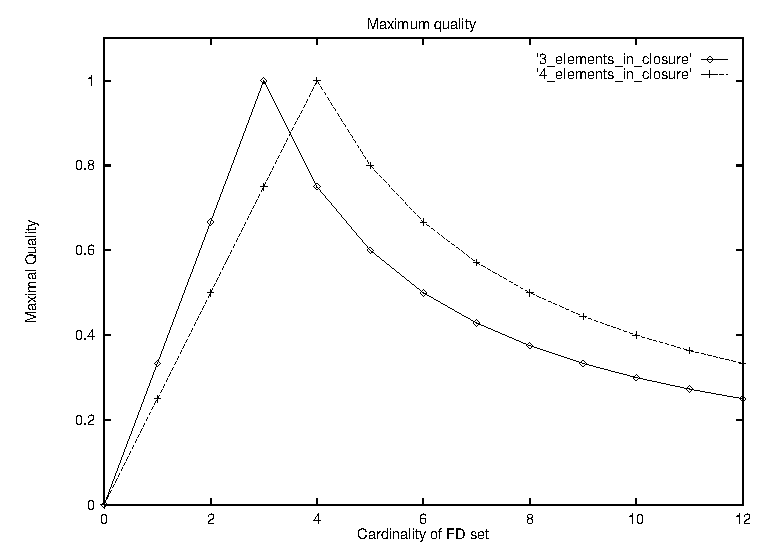
\includegraphics{../Quality/qual2.eps}}}
\caption{\label{graph:simquality}{Max Quality for FD sets with 3 and 4
elements in closure}}
\end{figure}

\begin{definition}[Similarity Measure]
\begin{rm}
Given two sets of FDs, F and G over R, we define the measure of
their similarity as:
\begin{displaymath}
sim({\rm F}, {\rm G}) = \frac{\mid {\rm CL(F)} \cap {\rm CL(G)} \mid}{\mid {\rm CL(F)} \cup {\rm CL(G)} \mid }
\end{displaymath}
\end{rm}
\end{definition}

We now seek to characterise the monotonicity properties of $sim$ with respect
to F and G. In equation~\ref{eq:f_xy} we consider the maximum
possible values of $sim$ where one FD set F is fixed, containing $n$
elements in CL(F). Any other FD set G
containing $k$ elements in CL(G) has a maximal quality, 
if all FDs in G are in F
whenever $k \le n$, and if all FDs in F are in G whenever $k > n$.
In Figure~\ref{graph:simquality} we show 
these variations for two fixed FD sets with 3 and 4 respective
elements in their closure.

\begin{equation}\label{eq:f_xy}
sim_F({\rm G}) = \left\{ \begin{array}
		{l@{\quad:\quad}ll}
\frac{n}{k} & n \le k & \quad\mbox{when}\quad {\rm G}^\star \supseteq
		{\rm F}^\star\\ 
\frac{k}{n} & n > k   & \quad\mbox{when}\quad {\rm F}^\star \supset
		{\rm G}^\star\\ 
			\end{array}	\right.
\end{equation}

The similarity measure is monotonically increasing and if a {\em
core}, or intersection, of the two FD sets is
increased by two different amounts, $m$ and $k$, where $m \le k$, then
the value of similarity is larger for the larger core size
increase. We now define some axioms of this similarity measure:
\begin{enumerate}
\item $sim({\rm F}, {\rm F}) = 1$
\item $sim({\rm F}, {\rm G}) = sim({\rm G}, {\rm F})$
\item $sim({\rm F}, {\rm G}) = 0$, if F$^\star \cap G^\star = \emptyset$
\item $sim({\rm F}, \emptyset) = 0$
\item $sim({\rm F}, {\rm G}) = \frac{|{\rm CL(F)}|}{ |{\rm CL(G)}|}$, if F$^\star \subseteq$ G$^\star$
\item  $sim({\rm F},{\rm G}) \le sim({\rm G},{\rm H})$ if F
$\subseteq$ H and H $\Delta$ F $\in$ G. 
\end{enumerate}

Information concerning related similarities can now be formed. Assume we
have three sets of FDs, F, G, and H, and that F is
fixed. Now, if $sim_{\rm F}$(G) = 0 and 0 $<$ $sim_{\rm F}$(H) $<$ 1
then we know 
that $sim({\rm G},{\rm H}) <$ 1 given that there is a similarity between F and
H. Essentially, this is stating that the core of F and H cannot 
form any part of the core of G and H. Using 
knowledge of the measure itself allows for inferences to be drawn
easily based on the input FD set and resulting values of the
measure. We have briefly
presented an overview of a similarity measure for FD sets. In
Chapter~\ref{chap:numdep} we define a metric based on the lattice
properties of NDs, used within our work on indefinite relations.

\subsection{Relational Database Sampling Procedures}\label{subsec:dat_samp}
\index{Sampling}
\index{Sample Size}
\index{PAC-learning}

Many real-world databases are too large to consider applying standard
data mining algorithms to. Therefore, as a solution, sampling from
such databases has been promoted \cite{km94,toi96b}. Samples drawn
from a large database are mined for dependencies which are then
associated with error and confidence thresholds based on the size of
the sample in relation to the the database. Alternatively, results
obtained from the mining of a sample may be verified against the
database as a whole. In this manner sampling is a necessary trade-off
between accuracy and efficiency of results.

\medskip

\cite{km94} addresses the problem of finding a suitable sample
size. This is presented within a PAC-learning framework
\cite{val84}. Based on an error measure, akin to the similarity
measure presented in Section~\ref{subsec:rev_fd_sim} or $g_3$ of
Table~\ref{tbl:fd_approx},  sampling is used to detect all sentences
which have an 
error (or 1 - similarity) less than a given threshold
$\epsilon$. The probability that at least one sentence with an error
greater than $\epsilon$ will not be formed is given by $\delta$, the
confidence parameter. FDs which hold are, obviously, never detected as
false. \cite{toi96b} presents sampling within an exact discovery
framework for association rules using a sample to find a superset of
frequent associations subsequently verified by one pass over the
database.


\subsubsection{Resampling in Statistics}
\index{Resampling}
\index{Bootstrap Resampling}
\index{Bootstrap Resampling!example}
Statistical methods have evolved rapidly over
the last 30 years, not least due to the harnessing of increasing
computational power.  In the 70's statistical modelling was based upon
decomposing the data into a structure and noise.  In the 80's
non-parametric 
processes such as the {\em jackknife} were developed where $n$ or more
(possibly) correlated estimates of the quantity of interest are
replaced by pseudovalues. Linear regression takes a linear combination
of the available values whereas non-parametric models keep the data
around and use it for estimating the response class of a new point.


The bootstrap \cite{efro79,de83,et93} is a data driven
simulation method for estimating the sampling distribution of a
statistic. It is a computationally 
intensive procedure that has been shown to provide good results which
would not have been capable of being readily generated more than 30 years ago.
In our experience, resampling has not previously been 
applied to solve database problems such as the consistency problem.
Declining computational cost is altering the face of statistical analysis
entailing a domino effect in other fields so that computer
intensive statistical methods such as the bootstrap will become much
more prominent in many areas of computer science over the next few years.
Figure~\ref{rev:bootstrap} shows how the
bootstrap procedure may be applied to an indefinite relation $r$. The
sample in the figure will consist of $n$ possible worlds, each
satisfying an ND set. We now introduce bootstrap resampling with a
simple example; resampling indefinite relations is formalised in
Chapter~\ref{chap:consistency}. 

\begin{figure}[ht]
\centerline{\scalebox{0.7}{{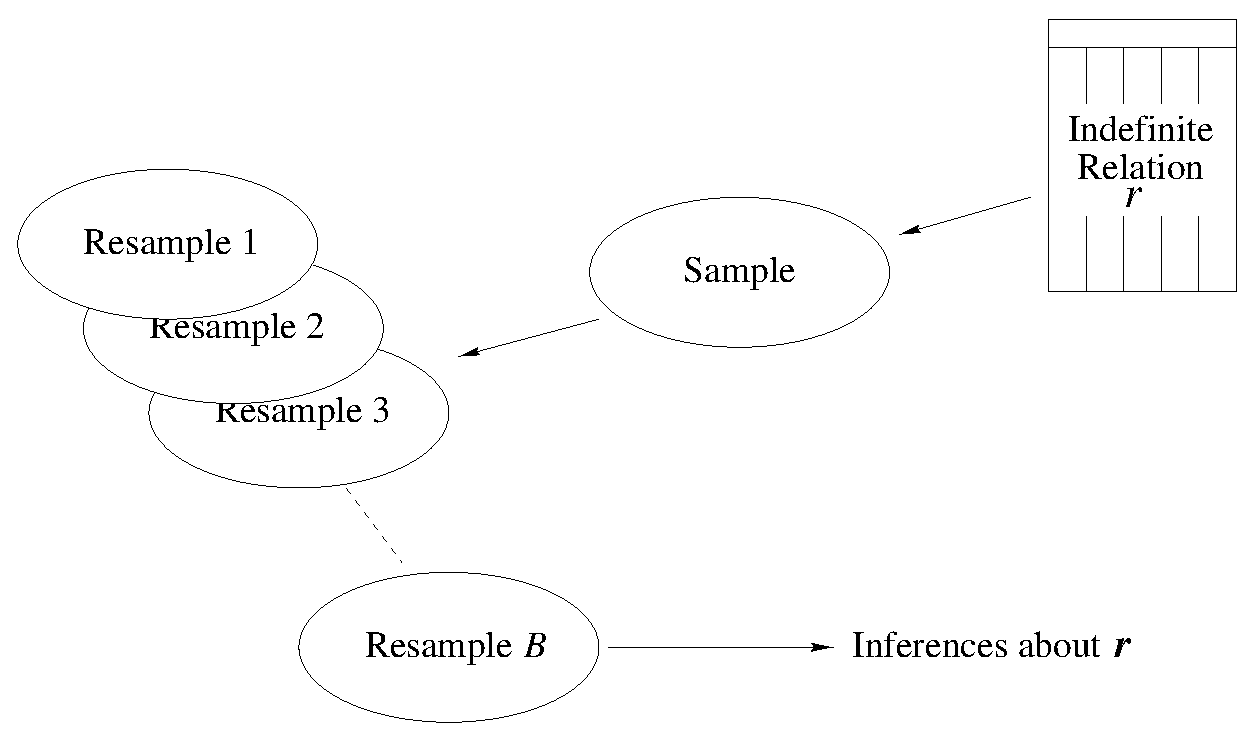
\includegraphics{review/bootstrap.eps}}}}
\caption{\label{rev:bootstrap} The Bootstrap Procedure as applied to an
indefinite relation with a Bootstrap Replication size (BRS) $B$}
\end{figure}

The following example is used for instruction and is similar
to one described in \cite{et93} but with a business 
application.
If we have a relation depicting the number of clients in 
two different companies with a number of the employees in
each company as in Table~\ref{table:3.01} then we can form a ratio of
success $\hat{\theta}$ based on the number of clients 
for the respective number of employees, given as follows:

\begin{displaymath}
\hat{\theta} = \frac{230 / 15746}{299 / 13430} = 0.66
\end{displaymath}

{\line
\begin{table}[ht]
\begin{center}
\begin{tabular}{|c|c|c|} \hline
Company & Clients & Employees \\ \hline
HAL co.	& 230		& 15746 \\
JCN co. & 299 		& 13430 \\ \hline
\end{tabular}
\end{center}
\caption{\label{table:3.01} Company Data Relation}
\end{table}
}

So we can say that HAL co. is only 66\% as successful as JCN co. Yet
this is only an estimated ratio. To apply a bootstrap procedure to
the above data we can create two sample populations for each
company and then, if we assume an optimal client - employee ratio is
1 to 10 then we construct each sample population with 230 clients and
(1575 - 230) employees and 299 clients and (1343 - 299) employees respectively.
Now if we draw with replacement a sample of 1575 subjects and 1343 subjects
we can form what is known as a bootstrap replicate sample
$\hat{\theta^\star}$. We can now repeat this say, 1000 times, to
obtain standard deviation values or other statistics which are based
on the distribution found and not naive assumptions on the distribution.

\smallskip

The majority of bootstrap applications in the statistical domain use
resampling due to the unavailability of the complete domain. Likewise,
in an indefinite relation, although we potentially have access to all
possible worlds, there are generally too many to examine them all. We
employ resampling in a dynamic manner on increasing sample sizes,
elaborated upon in Chapter~\ref{chap:consistency}. 

\section{Discussion}


Within the limits of our experience, there has
been no work on the data mining of relations containing indefinite
information, possibly due to the lack of availability of indefinite data.
Catalytic relations, those that are essentially the join of
two or more relations, provide a possible avenue for indefinite
information data mining if the join performed does not create the
cartesian product but instead creates disjunction within cells which
do not agree on their attributes, referred to in
Section~\ref{subsec:tl_catdm}. 

\medskip

The work of \cite{Via87,Via88} was seminal in the field of temporal
dependencies. Possible extensions discussed herein for NDs
in~\ref{subsec:temdat} warrant
further study. Nearly all work on dependency mining
\cite{Mann92,km95,sf93,bb95,hkp98} presents studies of the efficiency
of dependency mining, frequently noting that large number of
dependencies were discovered in relations. For example, \cite{sf93}
reports the discovery of 1191 FDs in a relation with 471 tuples over
17 attributes. Obviously the majority of these FDs discovered will
be near trivial due to large left hand side attribute sets functioning as
keys. We remark that there has been little work assessing the
real value of FD discovery in the data mining process. Such
potentially meaningless FDs also motivate the use of a user supplied
template to 
define FD approximations to dependencies which the user is interested
in.  

\medskip

From the work of \cite{mt96,bt98} we note the required restriction to
simple pattern discovery otherwise an NP-complete problem is
faced. Therefore it is necessary to restrict the discovery process. We
choose, in Chapters~\ref{chap:templog} and~\ref{chap:tempresult}, to
restrict our discovery to patterns which correspond to temporal
properties \cite{mp92}. We cite the work of
\cite{dlm98} and \cite{bt98} as having closely related goals to our
own work though 
their methodologies are different.





